% !TeX root = ../../Book1.tex
% 纲要标题：## 第6章　曲面的拓扑分类
% 纲要位置：几何学计划纲要.md，第 315 行。
% 正文状态：初稿；尚未正式审核。

% 纲要内容开始
% 
% > 本章目标与证明范围：把三角剖分、标准模型的存在和分类不变量的唯一性作为三个独立证明阶段。主范围为紧拓扑曲面，带边界情形同时处理；不把高维流形三角剖分问题混入本章结论。
% 
% 纲要内容结束

\chapter{曲面的拓扑分类}
\label{g1:ch:06}
\BookChapterNumber{g1:ch:06}

\begin{chapterabstract}
	一张紧曲面可以由有限个三角形拼成，继而化为球面上添若干手柄或交叉帽、再挖去有限个圆盘的模型。本章分别证明这两个存在性结论，再用可定向性、Euler 示性数和边界分支数说明模型的唯一性。三角剖分从纯拓扑坐标出发，先建立平面 Jordan--Schoenflies 定理与简单弧的直化；多边形约化则通过具体的切割粘合完成。最后讨论曲线的邻域、切开后的曲面与裤分解，为后续几何结构提供拓扑模型。
\end{chapterabstract}

\begin{learninggoals}
	\begin{itemize}
		\item 分清内点、边界点和闭曲面的含义，用绕数定义局部定向，并说明定向如何沿坐标图相容。
		\item 从平面分离与延拓证明出发，整理有限圆盘覆盖，构造紧拓扑曲面的有限三角剖分。
		\item 用生成树把剖分化为边配对多边形，说明每一步切割、重粘与封盘为什么保留所需拓扑信息。
		\item 抽取手柄和交叉帽，处理两者混合的情形，得到带边界的全部标准模型。
		\item 通过定向覆盖、Euler 示性数和边界分支数证明分类唯一性，并以基本群展示作独立核验。
		\item 判断曲线的一侧或两侧、分离或非分离，计算切开后的类型并构造可定向负 Euler 示性数曲面的裤分解。
	\end{itemize}
\end{learninggoals}

上一章已经算过环面和若干多边形商空间的基本群。但列出几个模型，并不等于知道所有曲面都在名单之中。即使每一点附近都是圆盘，把局部圆盘接成整体时仍可能产生复杂的环路；而一个基本群计算正确，也尚未给出从原曲面到某个模型的同胚。本章要回答的正是：紧曲面的名单能否列全，名单中的参数又能否唯一确定？

\ProseParagraphBreak

证明分成三个阶段。首先把任意紧拓扑曲面化为有限的三角形拼接；其次用切割和粘合整理这些有限材料，得到标准模型；最后找出同胚必须保持的量，区分模型。第一阶段需要认真对待连续曲线，因为拓扑坐标并没有导数，两条曲线的交点也未必有限。第二阶段则要追踪边的方向和粘合参数，不能只对边字作代数变形。第三阶段使用的 Euler 示性数，要先证明不依赖所选剖分，才能承担分类不变量的作用。

\ProseParagraphBreak

本章的曲面均为 Hausdorff、第二可数的二维拓扑流形，允许有边界；分类定理讨论紧曲面，并先逐个处理连通分支。用到上一章的圆周基本群时，会重新指出绕数的作用；用到覆盖分类、有限图的基本群和附着圆盘公式时，也会标出相应结论。平面拓扑与三角剖分部分的证明依据见 Thomassen 的论文\cite[Sections 2--4]{Thomassen1992}。希望从另一种教材组织方式复习紧曲面，可参见 Lee 的著作\cite[Chapter 6]{Lee2011Topological}。

% !TeX root = ../../Book1.tex
% 纲要标题：### 6.1 曲面与局部组合结构
% 纲要位置：几何学计划纲要.md，第 319 行。
% 正文状态：初稿；尚未正式审核。

% 纲要内容开始
% 
% * 内点、边界点与连通分支
% * 局部圆盘的相容缩小
% * 定向的局部定义
% 
% 纲要内容结束

\section{曲面与局部组合结构}
\label{g1:sec:0601}

球面、环面和圆盘在大部分点附近看起来都像一小块平面，差别在于这些小块怎样接成整体。圆盘的边缘还需要另一种局部模型：只能向一侧延伸的半平面。本节先把这两种点的区别、局部邻域的控制和定向说清楚。这里没有切向量，也没有坐标变换的导数；判断方向将使用上一章已经建立的绕数。

\subsection{内点、边界点与连通分支}
\label{g1:subsec:0601:01}

\begin{definition}[拓扑曲面]\label{g1:def:topological-surface}
	设 \(M\) 为 Hausdorff、第二可数的拓扑空间。若每个点都有一个开邻域 \(U\)，同胚于闭半平面
	\[
		\mathbb H^2=\{(x,y)\in\mathbb R^2:y\ge0\}
	\]
	中的相对开集，则称 \(M\) 为允许带边界的\term[tuopuqumian]{拓扑曲面}[topological surface]。这样的同胚 \(\varphi:U\to\varphi(U)\subseteq\mathbb H^2\) 称为\term[zuobiaotu]{坐标图}[coordinate chart]。当 \(\varphi(p)\) 的第二坐标大于零时，称 \(p\) 为内点；等于零时，称 \(p\) 为曲面的边界点。所有边界点组成的集合记为 \(\partial M\)，内点集记为 \(M^\circ\)。
\end{definition}

定义暂时用某张图区分两类点。必须证明它不随换图改变，否则 \(\partial M\) 就不是空间本身的性质。平面圆盘去掉中心后有不能缩掉的环路，半圆盘去掉直边中心后却没有；这提供了一个不依赖坐标名称的判断。

\begin{proposition}[边界的内在性]\label{g1:prop:boundary-invariance}
	在允许带边界的拓扑曲面中，一个点不可能在一张坐标图中为内点、在另一张图中为边界点。任一曲面同胚 \(f:M\to N\) 因而满足 \(f(\partial M)=\partial N\)。内点集开，边界集闭；\(\partial M\) 在子空间拓扑下是一维无边界拓扑流形。
\end{proposition}
\begin{proof}
	假设 \(p\) 同时有两种图。先在内点图中取以 \(p\) 为中心的坐标开圆盘 \(B\)，使它包含于两图的共同定义域；再在边界图中取以 \(p\) 为直边中心的坐标开半圆盘 \(D\subset B\)；最后取内点图中更小的同心圆盘 \(B'\subset D\)。选 \(z\in B'\setminus\{p\}\) 为共同基点。包含映射给出
	\[
		\pi_1(B'\setminus\{p\},z)\longrightarrow
		\pi_1(D\setminus\{p\},z)\longrightarrow
		\pi_1(B\setminus\{p\},z).
	\]
	两端的群都是 \(\mathbb Z\)，而复合为同构：同心穿孔圆盘沿半径收缩到小圆周，包含映射把绕一周送到绕一周，所用计算是\cref{g1:thm:circle-fundamental}。中间的群却平凡，因为穿孔半圆盘沿半径形变收缩到一条闭半圆弧，后者同胚于闭区间而可缩。这与复合同态为同构矛盾。

	同胚将坐标图带到坐标图，故保持两种点。内点有完全由内点组成的小圆盘邻域，所以 \(M^\circ\) 开，\(\partial M\) 闭。在边界图中，刚证的内在性说明边界恰对应直边上的一个开区间；这些限制图给出 \(\partial M\) 的一维无边界流形结构。
\end{proof}

这里的 \(\partial M\) 是曲面的内在边界，不是任意嵌入下的子集边界。例如圆盘 \(D^2\) 的曲面边界是 \(S^1\)，球面 \(S^2\) 的曲面边界为空；但把 \(S^2\) 放在 \(\mathbb R^3\) 中，它作为子集的拓扑边界是整个 \(S^2\)。第四章的 \(\partial_X A\) 仍指后一种依赖环境的边界。紧且边界为空的曲面称为\term[biqumian]{闭曲面}[closed surface]；“闭”在这里同时包含紧性，不能只理解为某个环境中的闭子集。

\begin{proposition}[分支与边界圆周]\label{g1:prop:boundary-circles}
	允许带边界的拓扑曲面局部道路连通，其连通分支就是道路分支，并且开。紧曲面只有有限个连通分支，其边界是有限多个彼此不交的圆周的并。
\end{proposition}
\begin{proof}
	小圆盘与小半圆盘都道路连通，且可以任意缩小，故曲面局部道路连通。由\cref{g1:thm:locally-path-components}，两种分支相同并且开。若曲面紧，用这些开分支覆盖它，只能有有限多个分支。边界闭，因而在紧曲面中紧；上命题又说明它是一维无边界流形。

	下面补上所需的一维事实，不预设一维流形分类。设 \(C\) 为紧的一维无边界流形。在每一点选取一段嵌入的闭区间，使该点落在其中部；由紧性，有限条闭区间的内部覆盖 \(C\)。把这些区间的所有端点组成有限集 \(P\)。每条区间去掉 \(P\) 后只有有限个开小段。因此 \(C\setminus P\) 只有有限个连通分支：它由有限个这样的连通小段覆盖。

	任取一个分支 \(J\) 和其中一点，选择覆盖该点的一个区间内部 \(U\)。由于 \(U\) 的两个端点都已删去，\(U\setminus P\) 在 \(C\setminus P\) 中既开又闭，故 \(J\) 完全落在其中一段内。于是 \(J\) 本身就是一个开区间，它的两端在 \(P\) 中。这样 \(C\) 成为有限图；每个顶点的区间邻域恰有左右两个半边，所以顶点的度数为二。从任一边出发沿唯一的下一条边继续，有限性迫使回到起点，且不能遗下同一连通分支中的其他边。因此每个连通分支是一个有限循环图，同胚于 \(S^1\)。应用于 \(C=\partial M\) 即得结论；空边界对应零个圆周。
\end{proof}

这个结论允许我们先分类连通紧曲面，再取有限不交并。以后用 \(b\) 记边界圆周数；它是曲面同胚必须保留的非负整数。

\subsection{局部圆盘的相容缩小}
\label{g1:subsec:0601:02}

一张坐标图不能覆盖整个环面，但在已有坐标图里，可以预留一圈余地后再动手修改曲线。这种“较小集合的闭包仍在较大坐标图中”的控制，会防止局部切割碰到图的边缘。此时相容指拓扑包含和覆盖关系，不预设坐标变换可微。

\begin{lemma}[带余量的坐标圆盘]\label{g1:lem:nested-surface-charts}
	设 \(M\) 为允许带边界的拓扑曲面，\(p\in M\)，\(O\) 为 \(p\) 的开邻域。可以在同一坐标图中选取三个相似的闭圆盘或闭半圆盘 \(K_1,K_2,K_3\)，使
	\[
		p\in\operatorname{Int}_M K_1,\qquad
		K_1\subset\operatorname{Int}_M K_2,\qquad
		K_2\subset\operatorname{Int}_M K_3,\qquad K_3\subset O.
	\]
	半圆盘的直边位于 \(\partial M\)。若 \(M\) 紧，可以选有限组这样的集合，使最小各片的相对内部覆盖 \(M\)。
\end{lemma}
\begin{proof}
	先限制坐标图到 \(O\) 内。在内点处，将坐标中心平移到原点，选闭球完全落在坐标像内，再取三个严格递增的小半径。在边界点处，对半平面取以直边上的坐标点为中心的三个闭半球。其直边中部在 \(M\) 中仍是相对内部点，因为半球本来就只需要包含半平面内的邻域。

	这些闭圆盘或半圆盘的坐标原像紧；\(M\) 为 Hausdorff，所以它们在 \(M\) 中闭，闭包关系与坐标中的关系一致。这说明每一级都保留了所需余量。对所有 \(p\) 先作选择，最小各片的内部成为开覆盖，紧性再给出有限子覆盖。
\end{proof}

每一点都有紧邻域，所以曲面局部紧。由\cref{g1:cor:lch-second-countable}，Hausdorff、第二可数与局部紧性保证存在相容距离；本章在需要控制网格大小时固定其中任意一个。距离的数值不是新的曲面不变量，它只帮助把“充分小”写成统一的有限条件。特别是对紧曲面的有限坐标覆盖，\cref{g1:lem:lebesgue-number}提供正数 \(\delta\)，使直径小于 \(\delta\) 的集合完全落入某一坐标图。

\ProseParagraphBreak

还需注意：两张图中的圆看起来都很规则，它们在重叠处却可能无限次相交。坐标变换目前只是同胚，不能用“稍微移动就横截”代替证明。下一节将在平面中建立简单曲线和简单弧的具体控制，再把有限圆盘覆盖整理成有限曲线网。有限覆盖本身尚不等于有限三角剖分。

\subsection{定向的局部定义}
\label{g1:subsec:0601:03}

在欧氏平面中，“逆时针”有确定意义。换到另一张拓扑坐标图后，一个小圆可能变成非常不规则的简单闭曲线，但它围绕像点的绕数仍有意义。对不经过 \(a\in\mathbb R^2\) 的环路 \(\gamma\)，定义
\[
	w(\gamma,a)=w\left(t\longmapsto
	\frac{\gamma(t)-a}{\lVert\gamma(t)-a\rVert}\right).
\]
右边是\cref{g1:thm:circle-fundamental}的圆周绕数。起点不必为 \(1\)：把角度提升的终值减去初值即可，改变初始角度不会改变这个整数。移动基点的环路同伦仍保持总角度增量，亦可由\cref{g1:prop:moving-basepoint}和 \(\mathbb Z\) 的交换性得到。

\begin{proposition}[平面换图的局部方向符号]\label{g1:prop:orientation-local-sign}
	设 \(U,V\subseteq\mathbb R^2\) 为开集，\(f:U\to V\) 为同胚。对 \(x\in U\)，取以 \(x\) 为中心、闭包包含于 \(U\) 的小圆，按逆时针参数化为 \(\gamma_x\)。整数
	\[
		\varepsilon_f(x)=w(f\circ\gamma_x,f(x))
	\]
	与小圆半径无关，只能等于 \(1\) 或 \(-1\)，且关于 \(x\) 局部常值。对可复合的同胚，有
	\[
		\varepsilon_{g\circ f}(x)=\varepsilon_g(f(x))\,\varepsilon_f(x),
		\qquad \varepsilon_{\operatorname{id}}=1.
	\]
\end{proposition}
\begin{proof}
	同心小圆可沿半径在 \(U\setminus\{x\}\) 中变形到彼此，因此它们的像有相同绕数。为证明这个数的绝对值为一，取以 \(x\) 为中心的开圆盘 \(B\)，再取以 \(f(x)\) 为中心的圆盘 \(D\)，使 \(\overline D\subset f(B)\)，最后取以 \(x\) 为中心的圆盘 \(B'\)，使 \(f(B')\subset D\)。穿孔空间上的同态组成
	\[
		\pi_1(B'\setminus\{x\})\xrightarrow{\,f_*\,}
		\pi_1(D\setminus\{f(x)\})\longrightarrow
		\pi_1(f(B)\setminus\{f(x)\}).
	\]
	这里各群都是无限循环群：前两者由径向收缩得到，第三者由同胚 \(f\) 与 \(B\setminus\{x\}\) 得到。复合同态是同构，因为它就是 \(f\) 复合同心穿孔圆盘的包含同构。把两个同态写成整数乘法，其乘数的乘积为 \(1\) 或 \(-1\)，所以两个乘数都为 \(1\) 或 \(-1\)。第一个乘数正是所定义的绕数。基点可沿相应小区域中的道路对齐；循环群的内自同构平凡，不影响这些整数。

	证明局部常值时，固定一条围住 \(x\) 的坐标圆 \(C\)，其闭圆盘包含于 \(U\)。对圆盘内部任何 \(y\)，\(C\) 都代表绕 \(y\) 一周的类：以 \(y\) 为中心向一个充分小的圆作径向收缩，所有径向线段留在这个凸圆盘中。因此
	\[
		\varepsilon_f(y)=w(f\circ C,f(y)).
	\]
	当 \(y\) 沿圆盘内部的道路移动时，\(f(y)\) 始终避开 \(f(C)\)，上式的归一化方向连续变化，给出圆周环路的同伦。于是整数不变，证明局部常值。

	最后在 \(x,f(x),g(f(x))\) 处逐级取充分小的圆盘。穿孔小邻域中的基本群均由正向小圆指定生成元；\(f_*\) 和 \(g_*\) 分别是乘以相应符号，复合便乘以两者之积。恒等映射显然把正向圆保留为正向圆。
\end{proof}

若换图涉及边界，先在半圆盘的内点部分使用上述符号。这个部分连通，所以符号恒定；把相同符号赋给其直边点。缩小半圆盘不会改变符号，乘法公式也通过内点的公式延续到边界。这里不把半圆盘边界上的点当作平面内点来计算绕数。

\begin{definition}[局部定向与曲面的定向]\label{g1:def:surface-orientation}
	在固定点 \(p\)，把一张坐标图 \(\varphi\) 和一个符号 \(s_\varphi\in\{1,-1\}\) 配在一起；若另一对 \((\psi,s_\psi)\) 满足 \(s_\psi=\varepsilon_{\psi\circ\varphi^{-1}}(\varphi(p))s_\varphi\)，便把这两对视为等价。符号的乘法公式保证这是等价关系，每个点恰有两个等价类，称为该点的两个局部定向。它们记录同一方向在不同坐标中的写法。
	设 \(M\) 为允许带边界的拓扑曲面。在每个点的坐标图中标记一个符号 \(s_\varphi\in\{1,-1\}\)，其中符号在图内局部常值；若在任意两图交叠处都满足
	\[
		s_\psi(p)=\varepsilon_{\psi\circ\varphi^{-1}}(\varphi(p))\,s_\varphi(p),
	\]
	并将满足此关系的局部描述视为同一选择，则称这些相容选择为 \(M\) 的一个\term[dingxiang]{定向}[orientation]。存在定向的曲面称为\term[kedingxiang]{可定向}[orientable]，否则称为不可定向。直观上，符号 \(1\) 选定图中的逆时针方向，符号 \(-1\) 选定相反方向。
\end{definition}

只需在覆盖 \(M\) 的一组坐标图上给出相容符号：乘法公式保证它们唯一地确定所有其他图中的符号。这个定义不要求选择一个全局坐标系；它要求的是各处的局部方向能接在一起。对连通可定向曲面，定向恰有两个，因为两个定向在每点的符号比值为局部常值的 \(\pm1\)，在连通空间上只能恒定。

\begin{example}[平面方向与环面的定向]\label{g1:exm:torus-local-orientation}
	平移与旋转把正向小圆送到正向小圆，故方向符号为 \(1\)；反射 \((x,y)\mapsto(x,-y)\) 的符号为 \(-1\)。在环面模型 \(\mathbb R^2/\mathbb Z^2\) 中，充分小的投影圆盘作为坐标图，重叠处的坐标变换为整数平移。因此所有这些图均选符号 \(1\) 就得到环面的定向。将全部符号同时取反，得到另一个定向。
\end{example}

对平面中带边界的区域，正定向规定沿边界行走时区域留在左侧。若取半平面 \(y\ge0\) 的正定向，直边上的正向就是 \(x\) 增大的方向。定向相容的换图保留这个选择：把一段直边与内侧一条简单弧合成小半圆盘的边界，边界的行走方向由内点的正向小环路决定，换图符号为正时这个方向不变。下一节的简单弧直化会给出这个边界描述的圆盘坐标。反转曲面定向时，各边界圆周的诱导方向也同时反转。

% !TeX root = ../../Book1.tex
% 纲要标题：### 6.2 紧曲面三角剖分的证明
% 纲要位置：几何学计划纲要.md，第 325 行。
% 正文状态：初稿；尚未正式审核。

% 纲要内容开始
% 
% * 平面 Jordan–Schoenflies 定理与简单弧直化
% 
%   在局部平面图中先建立 Jordan–Schoenflies 的平面 Jordan 曲线版本，以及圆盘内适当嵌入简单弧的直化与延拓引理，再处理有限曲线网。三角剖分的主范围为紧、Hausdorff、第二可数的拓扑二维流形，边界允许存在；平面拓扑引理为本章明确的证明任务，不预设曲面已有光滑图册，也不调用高维三角剖分结论。
% 
% * 交叠边界的局部有限交叉
% * 由曲线网得到有限胞腔分解
% * 圆盘胞腔的三角化
% * 同痕后的公共细分与 Euler 示性数不变性
% 
% 纲要内容结束

\section{紧曲面三角剖分的证明}
\label{g1:sec:0602}

形成有限三角剖分，需要把坐标图中的曲线整理成有限的边与顶点。简单闭曲线可能处处没有切线，圆盘边界也可能无限相交；平面中的分离与直化结论使我们能够逐个调整边界，同时保留圆盘覆盖。平面部分采用有限图与逐次加密的构造；这条证明思路见\cite[第2--4节]{Thomassen1992}。

\subsection{平面 Jordan–Schoenflies 定理与简单弧直化}
\label{g1:subsec:0602:01}

这里的简单弧是 \([0,1]\) 的嵌入像，\term[Jordanquxian]{Jordan 曲线}[Jordan curve]是 \(S^1\) 的嵌入像。\footnote{Camille Jordan（1838--1922），法国数学家，研究群论与拓扑。}嵌入的参数映射可以非常不规则；整个论证只用连续性和单射性。先给出后面所需的平面分离与有限图结论。

\begin{lemma}[有限折线与平面图]\label{g1:lem:polygonal-plane-tools}
	下列事实成立。
	\begin{enumerate}
		\item 平面连通开集中的任意两点可以用一条简单折线连接。
		\item 简单闭折线把平面分成两个连通开集，其中一个有界；二者的边界都是这条折线。闭折线内部的一条简单折线弧若恰在两个端点与边界相交，就把内部切成两个区域，其边界分别由该弧与原边界的两段组成。
		\item 任意有限图在平面中的嵌入都可以重新画成边为折线的嵌入。完全二部图 \(K_{3,3}\) 没有平面嵌入；把一个平面图中的互不相交的有限树各收缩成一点，仍得到平面图。
		\item 若一个有限平面图连通、没有环边、没有割点，且至少有三个顶点（若原图有环边，先将环边细分，再检验这些条件），则它可以从任一圈开始，逐次加入两端在旧图上、内部与旧图不交的简单弧得到。若各边为折线，它的每个面以一个简单圈为边界。
	\end{enumerate}
\end{lemma}

\begin{proof}
	对于第一项，固定起点，把能用有限折线到达的点组成集合。小圆盘内可以添一条线段，所以这个集合及其补集在给定开集中都开；连通性说明它等于整个开集。有限条线段的交点和重叠端点只有有限个，把它们作为顶点得到有限图，删去回路便得到简单折线。

	对于第二项，先给出折线两侧的具体含义。在每条边的内部取窄矩形，在每个顶点取足够小的圆盘，使不相邻的这些小邻域不相交；顶点圆盘内只有两条相接的半径方向，可以沿这两条边的两侧分别绕过顶点。沿整个多边形走一周，得到两条互不相交的窄通路。平面补集中的任一点可以沿折线走向边界，取第一次接触以前的一小段，就到达这两条通路之一；若接触顶点，改在顶点圆盘中的相应扇形内行走。因此补集至多有两个分支。

	再证明两侧不能相通。从不在边界上的点向无穷远发一条射线，先让射线避开顶点且不平行于边，记录它与边界的交点数模 \(2\)。改变射线方向经过一个顶点时，两次交点同时出现或消失，或者一次交点换到相邻边，故奇偶性不变。沿不碰边界的短线段移动起点也不改变奇偶性：在扫过的窄四边形中，每段边界从边界进入还必须离开，交点变化为偶数。有限折线连接把这一结论推广到同一分支中的任意两点。跨过一条边的内部时奇偶性恰好改变，因此确有两个分支。足够大的圆外连通，故只有一个分支无界；窄通路同时说明边界上的每一点都在两分支的闭包中。对于内部弧，把它与边界的两段分别组成简单闭折线，重复奇偶性论证；弧的两侧不同，而每一侧都沿对应边界窄通路连通，恰好得到所说的两个区域。

	第三项的重新画法不要求原边可微。先给环边添一个顶点，使每条边有不同的端点。在每个顶点周围取互不相交的小圆盘，只截到与该顶点相接的边。对每条边取最后离开起点圆盘以后、随后第一次进入终点圆盘以前的闭子弧；这些子弧两两不交，因而有两两不交的开邻域。用第一项在各邻域内改画简单折线，并在顶点圆盘内用互不相交的径向线段接到顶点。\(K_{3,3}\) 包含一个六边圈和连接三对相对顶点的三条弦。在折线画法中，至少两条弦落在该圈的同一侧；它们的四个端点沿圈交错，与第二项的切分结论矛盾。有限折线树的细邻域可以由顶点小圆盘和边的细矩形组成；从叶边开始依次添加矩形和端点圆盘，每次仍是一个闭盘。在该闭盘内把树及其附着边改画成一颗星，就实现树的收缩。这也说明若一个图经过收缩互不相交的树能得到 \(K_{3,3}\)，原图便不能平面嵌入。

	最后证明第四项。已有一个没有割点的真子图 \(H\)。若剩余某条边的两端都在 \(H\) 中，可直接加入。否则，取 \(G\setminus H\) 的一个连通分支；它必须接到 \(H\) 的至少两个不同顶点，因为只有一个接点会成为 \(G\) 的割点。在该分支中选连接两个接点的最短路径，便得到所需的新弧。加入它仍没有割点，有限次便遍历全部边。从初始圈出发，每加入一条弧，它都位于某个旧面的内部；第二项说明它把该面分成两个以简单圈为边界的面。于是归纳得到最后的结论。
\end{proof}

下面两步把折线结论推广到任意连续弧和闭曲线。关键区别是：任意简单弧仍然不能隔断平面，而闭曲线确实会隔断。

\begin{lemma}[简单弧不分离平面]\label{g1:lem:arc-nonseparation}
	若 \(A\subset\mathbb R^2\) 是简单弧，则 \(\mathbb R^2\setminus A\) 道路连通。
\end{lemma}

\begin{proof}
	固定 \(x,y\notin A\)，取 \(d>0\)，使它们到 \(A\) 的距离都大于 \(4d\)。按参数把 \(A\) 分成有限段 \(A_1,\ldots,A_k\)，每段直径小于 \(d\)。不相邻的闭段互不相交，所以其间距离的最小值为正；取 \(0<\delta<d\) 小于这些距离。若只有一两段，直接任取这样的 \(\delta\)。在每段上取更细的点列，使相邻点间的子弧直径小于 \(\delta/8\)，并在每个点处画边长 \(\delta/2\)、边平行于坐标轴的正方形。记第 \(i\) 段所用正方形边界的并为 \(G_i\)，把有限交点添作顶点。

	相邻正方形的边界至少有两个公共点；由\cref{g1:lem:polygonal-plane-tools}最后一项，或直接删去任一顶点检查，\(G_i\) 没有割点。相邻的 \(G_i,G_{i+1}\) 包含同一个端点正方形；不相邻的图不交。每一对相邻图都包含在以公共弧端点为中心、半径 \(3d\) 的圆盘内，所以 \(x,y\) 位于这对图的无界面。

	需要一个有限图的观察：这种链状排列的图若把一点围在有界面内，必有一对相邻图已经把它围住。证明如下。由前一引理，整个并没有割点，各有界面的边界都是圈。若观察不成立，取围住该点的圈 \(C\)，使它所用图的最大下标 \(j\) 最小，再使 \(C\) 使用 \(G_j\setminus G_{j-1}\) 的边数最少。若 \(C\) 只在 \(G_{j-1}\cup G_j\) 内，已经矛盾；否则 \(C\) 在 \(G_{j-1}\) 上至少有两段。\(G_{j-1}\) 没有割点，故可取一条内部避开 \(C\) 的路径连接其中两段：在 \(G_{j-1}\) 中取连接两段的最短路径，并截去首次接触之前和末次接触之后的部分即可。它把 \(C\) 切成两个圈；点不在新路径上，必在其中一个圈的内部。该圈或者降低最大下标，或者减少所数的边，均与选择矛盾。

	因此 \(x,y\) 都位于 \(G=\bigcup_iG_i\) 的无界面。这个面是连通开集，可用简单折线连接两点。每一段 \(A_i\) 都被相应正方形覆盖，而每个正方形内部与 \(G\) 的无界面不交；故所得折线避开 \(A\)。
\end{proof}

\begin{theorem}[Jordan 曲线分离定理]\label{g1:thm:jordan-separation}
	任意 Jordan 曲线 \(C\subset\mathbb R^2\) 的补集恰有两个分支：有界分支 \(D\) 和无界分支 \(E\)，且 \(\partial D=\partial E=C\)。两分支都是道路连通的开集。
\end{theorem}

\begin{proof}
	先证至少有两个分支。取两条竖直支撑线，使 \(C\) 位于它们之间，在每条支撑线上取 \(C\) 的最高点 \(p_1,p_2\)。曲线分成从 \(p_1\) 到 \(p_2\) 的两段。在两支撑线之间再取一条竖线，这两段与该线都相交；沿该线找到两个相邻的、分别属于两段的交点 \(a,b\)，使开线段 \((a,b)\) 避开 \(C\)。这是可行的，因为两组交点是互不相交的紧集。另从 \(p_1\) 向上、经曲线上方的水平线、再降到 \(p_2\)，画一条内部避开 \(C\) 的折线 \(L\)。若线段 \((a,b)\) 的中点可以在补集中到达无穷远，它就可以接到 \(L\) 的内部；截取首次接触，所得连接弧的内部同时避开 \(C\)、\([a,b]\) 和 \(L\)。于是 \(C\)、\([a,b]\)、\(L\) 及这条连接弧组成一个 \(K_{3,3}\) 的细分：两类顶点分别是 \(p_1,p_2\) 与连接弧在 \([a,b]\) 上的端点，以及 \(a,b\) 与连接弧在 \(L\) 上的端点。这与\cref{g1:lem:polygonal-plane-tools}矛盾。因此补集不连通。

	对补集的任意分支 \(U\)，考察从 \(U\) 内出发、恰在终点接触 \(C\) 的折线。这些折线所能到达的端点在 \(C\) 中稠密。事实上，任取一个开子弧 \(J\subset C\)，\(C\setminus J\) 是简单闭弧；由\cref{g1:lem:arc-nonseparation}，可用避开该闭弧的折线连接 \(U\) 中的一点和另一个分支中的一点。它第一次离开 \(U\) 时只能碰到 \(J\)，这就给出一个所需的可达点。子弧可以任意缩小，稠密性随之成立。

	假设补集有三个分支 \(U_1,U_2,U_3\)，在曲线上选三段互不相交的短闭子弧 \(J_1,J_2,J_3\)。每个 \(U_i\) 中可以画一棵有限的折线树，分别接到三个 \(J_j\)，且除这些端点外避开 \(C\)：先用上一段选可达点，再在连通开集 \(U_i\) 内连接三条到达折线，删除多余回路。三棵树互不相交。把各树及每个 \(J_j\) 上连接三个接触点的最短子弧各收缩为一点，得到 \(K_{3,3}\)，仍与有限图引理矛盾。所以恰有两个分支。

	足够大的圆外是连通的，因此恰有一个无界分支。补集是开集，平面的连通开集道路连通。边界只能落在 \(C\) 上，而上述可达点在 \(C\) 上的稠密性说明 \(C\) 上每一点都属于每个分支的边界。
\end{proof}

\begin{lemma}[横切弧与有限弦网]\label{g1:lem:jordan-crosscuts}
	设 \(C\) 是 Jordan 曲线，\(D\) 是其有界补分支。若简单折线弧 \(P\) 的内部在 \(D\) 中，且两个端点是 \(C\) 上的不同点，那么 \(P\) 把 \(D\) 切成两个区域，边界分别由 \(P\) 与 \(C\) 的两段组成。设 \(G\) 为由 \(C\) 和 \(D\) 中有限条折线弧组成的连通有限图，将环边先作细分，并假设细分后的图没有割点。则 \(G\) 的每个有界面都以 Jordan 曲线为边界；在某个面中添加一条上述弧，恰好把该面分成两个。
\end{lemma}

\begin{proof}
	记 \(C\) 的两段为 \(A_1,A_2\)，\(C_i=P\cup A_i\) 的有界内部为 \(D_i\)。原曲线的无界外部 \(E\) 是避开 \(C_i\) 的连通无界集，故在 \(C_i\) 的外部。\(A_2\) 的内点属于 \(\overline E\) 又不在 \(C_1\) 上，因此也在 \(C_1\) 的外部；同理 \(A_1\) 的内点在 \(C_2\) 外部。于是 \(D_1\) 不碰 \(C\)，且不在 \(E\) 中，故 \(D_1\subset D\)，同理 \(D_2\subset D\)。

	\(D_1\) 连通且不碰 \(C_2\)，所以整体位于 \(C_2\) 的一侧。若 \(D_1\subset D_2\)，闭包包含关系将使 \(A_1\) 的内点落在 \(\overline{D_2}\)，与上一段矛盾。因此 \(D_1\cap D_2=\varnothing\)。在 \(P\) 的任一内点处取足够小的圆盘，使 \(P\) 在其中是一条折线直径；若恰为折点，先用扇形坐标把两段边变直。在这个小盘中，\(C_1,C_2\) 都只有同一段 \(P\)。Jordan 定理说明每个 \(D_i\) 都接近该点；两侧半盘连通，因此其中一侧属于 \(D_i\)。两内部互不相交，说明它们恰好占据相反的两侧。

	所以 \(D_1\cup P^\circ\cup D_2\) 在 \(D\) 中是开集。它也是 \(D\) 中的闭集，因为它等于 \((\overline{D_1}\cup\overline{D_2})\cap D\)。\(D\) 连通且这个集合非空，故它等于 \(D\)。这就证明 \(D\setminus P=D_1\sqcup D_2\)，并且各自边界正是 \(P\cup A_i\)。有限图部分再按\cref{g1:lem:polygonal-plane-tools}的逐次加弧构造归纳；这里每次只调用刚证明的横切弧结论。
\end{proof}

把 \(D\cup C\) 实现为闭圆盘，需要将边界上的对应延拓到内部。Jordan--Schoenflies 定理的构造同时细化原像和像中的网格，使两侧相邻点的控制在极限中都保留下来，从而得到连续且互逆的映射；\cref{g1:fig:double-mesh}给出构造的示意。\footnote{Arthur Sch\"onflies（1853--1928），德国数学家，研究拓扑与晶体群。}

% !TeX root = ../Book1.tex
\begin{figure}[htbp]
	\centering
	\begin{tikzpicture}[scale=0.88, every node/.style={font=\small}]
		\begin{scope}
			\draw[thick] (-2,-1.4) .. controls (-2.5,-0.2) and (-2.1,1.6) .. (-0.8,1.8) .. controls (0.2,1.4) and (1.1,2.1) .. (1.9,1.3) .. controls (2.4,0.3) and (1.8,-1.6) .. (0.9,-1.8) .. controls (-0.3,-1.4) and (-1.2,-2) .. cycle;
			\draw[GeometryBlue,thick] (-1.2,-0.9) rectangle (1.2,0.9);
			\foreach \x in {-0.6,0,0.6}{\draw[GeometryBlue] (\x,-0.9)--(\x,0.9);}
			\foreach \y in {-0.45,0,0.45}{\draw[GeometryBlue] (-1.2,\y)--(1.2,\y);}
			\draw (-1.2,0.9)--(-0.8,1.8);
			\draw (1.2,-0.9)--(0.9,-1.8);
			\node at (0,2.25) {原区域 \(D\)};
			\node[fill=white,inner sep=2pt] at (0,-0.2) {\(K_n\)};
			\node at (-1.8,1.7) {\(C\)};
			\node at (0,-2.3) {紧集附近的网格逐次变细};
		\end{scope}
		\draw[->,thick] (2.7,0.2)--(3.7,0.2);
		\draw[<-,thick] (2.7,-0.2)--(3.7,-0.2);
		\begin{scope}[xshift=6.4cm]
			\draw[thick] (-1.8,-1.8) rectangle (1.8,1.8);
			\draw[GeometryBlue,thick] (-1.2,-0.9) rectangle (1.2,0.9);
			\foreach \x in {-0.6,0,0.6}{\draw[GeometryBlue] (\x,-0.9)--(\x,0.9);}
			\foreach \y in {-0.45,0,0.45}{\draw[GeometryBlue] (-1.2,\y)--(1.2,\y);}
			\draw (-1.2,0.9)--(-1.8,1.8);
			\draw (1.2,-0.9)--(1.8,-1.8);
			\node at (0,2.25) {目标正方形 \(Q\)};
			\node at (0,-2.3) {再加密像侧，并把新弦复制回去};
		\end{scope}
	\end{tikzpicture}
	\caption{双向网格控制的示意。每次只在内部添加有限条弦；原边界上的对应保持不变。两边都要加密，才能保证极限及其逆都连续。图中的光滑边界只为示意，证明允许任意 Jordan 曲线。}
	\label{g1:fig:double-mesh}
\end{figure}


\begin{theorem}[Jordan--Schoenflies 定理]\label{g1:thm:jordan-schoenflies}
	任意两条平面 Jordan 曲线之间的同胚都可以延拓为整个平面的同胚。特别地，每条 Jordan 曲线及其有界补分支的并同胚于闭圆盘，而且给定的边界同胚可以一并延拓。
\end{theorem}

\begin{proof}
	先把给定边界同胚写成 \(f:C\to\partial Q\)，其中 \(Q\) 是正方形；若这个情形成立，对两条曲线分别构造到正方形的延拓再复合即可。记 \(D\) 为 \(C\) 的内部。我们构造一列有限弦网 \(G_n\subset\overline D\)、\(G'_n\subset Q\)，始终包含边界，内部边为折线。每个图没有割点，其删去边界后的部分连通；两图具有相同的顶点、边、面关系，边界对应始终是 \(f\)。在这个阶段只固定顶点的对应，不固定内部边上每一点的参数。

	从 \(D\) 可沿折线到达的边界点中选可数稠密集 \(A\)，这是\cref{g1:thm:jordan-separation}证明中得到的。取两个这样的点，用 \(D\) 中的简单折线连接，得到初始弦；在正方形内取对应弦。于是得到 \(G_0,G'_0\)。以后依次把 \(A\) 的各点加入顶点集：从新点沿到达折线走进 \(D\)，再连到旧图内部，截到第一次碰到旧图为止。它在某个旧面内成为一条新弦。在对应的正方形面内也可画出相应弦；该面内部连通，端点位于折线边或已有可达的边界点，先取端点处的小段，再用连通开集中的简单折线相接即可。\cref{g1:lem:jordan-crosscuts}保证两面以相同方式各分为两面。

	同时必须加密网格。令
	\[
		K_n=\{x\in\overline D:\operatorname{dist}(x,C)\ge 1/n\}.
	\]
	在 \(D\) 内加入有限个小正方形的边及其中的横、竖网格，使 \(K_n\) 被这些正方形的内部覆盖，且网格的每格直径小于 \(1/n\)。所有这些边与旧图的内部折线只有有限个交点，并与 \(C\) 不交。必要时添加有限条内部折线，使新图没有割点且内部连通。这个补充可以如下完成：先连接各分支；若有割点 \(v\)，在 \(v\) 两侧的分支中各取靠近 \(v\) 的点，在 \(D\setminus\{v\}\) 中用折线连接。连通开集删去一点仍连通，因为一条经过该点的折线可以在一个小圆盘内绕过它。把新交点作为顶点后，这条连接把割点处分开的块合并，使块数至少减少一；按有限图的块数归纳即可结束。每次新增弧都可拆成有限次在旧面内加弦，因而可以在 \(Q\) 中逐条复制其组合关系。

	接着反过来，在 \(Q\) 的内部加入足够细的有限网格，使到边界距离至少 \(1/n\) 的部分被直径小于 \(1/n\) 的网格包围；再把这些弦逐条复制回 \(D\)。新端点若落在已有边的内部，就在对应边上选一个新点，保持已有各点的次序；若在边界上，则选取 \(f(A)\) 中的点。可在边界附近略弯折网格末端以做到这一点，内部网格不受影响。仍用前一段的加弦过程补足连通性。后加的弦只细分已有面，不会破坏先前的网格。因此，对于原像与像两侧各自的每个内部紧集，以及每个 \(\varepsilon>0\)，从某一步起，紧集上每一点都位于一个由图中边组成的简单小圈内部，而这个小圈连同内部的直径小于 \(\varepsilon\)。若点恰在网格边或顶点上，就取环绕它的两行、三行小格的外框；把网格取得更细即可达到同一要求。

	把所有顶点及整个边界组成集合 \(F\)，相应集合记为 \(F'\)。构造给出双射 \(f_0:F\to F'\)，且两集合分别在 \(\overline D,Q\) 中稠密。它保持有限弦网中每个圈的内外关系：这在每次加弦时由横切弧引理保持。现在证明上述对应延拓为同胚。

	取 \(x\in D\)。在某个图中选围住 \(x\) 的内部圈 \(L\)，其对应圈 \(L'\) 也在 \(Q\) 内部。趋近 \(x\) 的 \(F\) 中点最终在 \(L\) 内，像点因而留在 \(L'\) 围出的紧区域中。任取其像点的两个聚点 \(y,z\)。若 \(y\ne z\)，利用像侧越来越细的网格，在 \(y\) 附近取两个互不相交的嵌套网格圈，它们都把 \(y\) 与 \(z\) 分开。对应的两个原像圈也互不相交，至多一个经过 \(x\)。取另一个圈 \(M\)；趋近 \(x\) 的点最终都在 \(M\) 的同一侧，像点也都在对应圈的同一侧，不可能同时趋近位于相反侧且不在圈上的 \(y,z\)。故像点只有一个极限，定义它为 \(h(x)\)。同样的论证对反向顶点对应成立，得到 \(k:Q^\circ\to D\)。这里聚点不会落在边界：环绕任一内部点的内部小圈及其对应圈已经把聚点限制在内部的紧区域。常值顶点序列也是允许的趋近序列，所以延拓在每个已有顶点上与 \(f_0\) 一致。

	这些延拓连续。给定 \(h(x)\) 的一个小邻域，取像侧两个互不相交的嵌套内部小圈，都把 \(h(x)\) 围在其中，并令闭内部落在该邻域；至少一个对应原像圈不经过 \(x\)，选取这一个。它必须围住 \(x\)，否则稠密顶点的对应违反内外关系。这个原像圈的内部便是 \(x\) 的一个邻域，整个邻域的像都落在给定小邻域中。同理 \(k\) 连续。两个复合映射在稠密顶点集上都是恒等映射，连续性给出 \(k\circ h=\mathrm{id}\)、\(h\circ k=\mathrm{id}\)。

	最后检查边界。设 \(x_m\in D\) 趋近 \(a\in C\)，而某个像子列趋近 \(b\in Q\)。若 \(b\in Q^\circ\)，内部圈及其原像紧区域迫使 \(x_m\) 留在 \(D\) 的一个紧子集，矛盾。故 \(b\in\partial Q\)。若 \(b\ne f(a)\)，在 \(C\) 上选两个 \(A\) 中的点 \(a_1,a_2\)，把 \(a\) 与 \(f^{-1}(b)\) 分开。它们最终都已加入图；因图的内部连通，可以在图内找到一条从 \(a_1\) 到 \(a_2\)、其余部分均在内部的简单弦。该弦及其对应弦把两边各分成两块。靠近 \(a\) 的点位于与 \(a\) 相邻的块，其像位于与 \(f(a)\) 相邻的块，后者的闭包不含 \(b\)，矛盾。因此 \(b=f(a)\)。紧性说明整个像序列都趋近 \(f(a)\)，从而 \(h\cup f\) 连续。它是紧空间到 Hausdorff 空间的连续双射，故为闭盘同胚。

	还要延拓到外部。先选各曲线内部的一点作为原点，对两平面作反演 \(x\mapsto x/\|x\|^2\)。每条曲线的外部连同无穷远点变成一条 Jordan 曲线的闭内部，原来的无穷远点对应原点。已经证明的闭盘延拓给出反演后两内部之间的同胚。可使它把原点映到原点：先把目标闭盘映到正方形，在正方形中从给定内部点与目标内部点分别向四角作扇形三角剖分，逐三角形的仿射映射给出固定边界、移动该点的同胚，再共轭回去。于是反演回去得到外部同胚，与内部同胚在原边界上相合。两部分的粘合连续，其逆也同样连续，故得到全平面同胚。
\end{proof}

\begin{lemma}[简单弧的直化与延拓]\label{g1:lem:proper-arc-straightening}
	平面简单弧的每个内点都有一个开矩形型邻域，使该邻域与原弧的交集在某个坐标下恰为水平直径。若 \(B\) 是闭 Jordan 盘，\(A\subset B\) 是简单弧，且 \(A\cap\partial B\) 恰为其两个端点，则 \(B\setminus A\) 有两个分支，闭包都是闭 Jordan 盘。给定把这两个端点送到另一闭盘中一条直径端点的边界同胚，可以延拓为把 \(A\) 送到该直径的闭盘同胚。
\end{lemma}

\begin{proof}
	先证局部结论。在所给内点 \(p\) 两侧各选一个短子弧。每个短子弧内都有从原弧补集沿线段可达的点：取靠近该子弧、但不在原弧上的点，再在原弧上选取离它最近的点，连接这两个点的开线段不碰原弧；起点取得足够近，最近点仍在指定短子弧内。补集由\cref{g1:lem:arc-nonseparation}连通，所以可用其中的折线连接两条到达线段，删去回路，得到一条与原弧只在所选两端点相交的简单弧。它与经过 \(p\) 的原子弧组成 Jordan 曲线。\cref{g1:thm:jordan-schoenflies}把这条曲线变成圆；再在圆上的对应点附近取普通矩形坐标，并缩小矩形以避开原弧剩下的紧集，就得到所求直化。

	对闭盘中的弧，将它分别与盘边界的两段组成 Jordan 曲线。重复\cref{g1:lem:jordan-crosscuts}的两个有界内部的论证：两内部不交且包含在 \(B\) 中；本引理刚证的局部直化使 \(A\) 每个内点附近都有两个半矩形，两个内部各占一侧；它们与 \(A^\circ\) 的并在 \(B^\circ\) 中同时开闭。因此它们恰为 \(B\setminus A\) 的两块，闭包只沿 \(A\) 相交。任取从 \(A\) 到目标直径、与给定两个端点相容的同胚。它与给定的边界同胚在两个子盘的边界上分别组成同胚；对两子盘应用\cref{g1:thm:jordan-schoenflies}并沿 \(A\) 粘合，便得到整个闭盘的同胚。
\end{proof}

这里有一个以后会反复用到的直接推论：位于一个平面图中的闭 Jordan 盘，其边界有双侧环带邻域。用全平面同胚把边界变成单位圆，再取 \(1-\varepsilon<r<1+\varepsilon\) 的逆像即可。有限条在一点相交、除此之外互不相交的弧也可以同时直化为有限条径向线段：先把两条组成的弧直化，再在各半盘内依次用上一引理直化其余弧；每次缩小中心邻域以避开各弧已经截去的紧尾部。因弧数有限，此过程结束后得到一个顶点小圆盘和互不相交的边矩形。因此，有限嵌入图具有由顶点盘、边带组成的细邻域。

\subsection{交叠边界的局部有限交叉}
\label{g1:subsec:0602:02}

现在回到曲面。紧性允许选有限个坐标圆盘，但不能保证它们的边界相交有限次；我们要改变边界，仍保留原来较小圆盘的覆盖性质。下面的论证只在一个坐标图内进行，因此同时适用于曲面上的有限条曲线。

\begin{lemma}[边界的有限化]\label{g1:lem:disk-boundary-regularization}
	设曲面 \(M\) 中有有限条简单曲线组成的嵌入有限图 \(G\)，以及一个坐标图内的三个闭 Jordan 盘
	\[
		B_0\subset\operatorname{int}B_1\subset B_1\subset\operatorname{int}B_2.
	\]
	存在闭 Jordan 盘 \(B\)，使 \(B_0\subset\operatorname{int}B\subset B\subset\operatorname{int}B_2\)，且 \(\partial B\) 与 \(G\) 只有有限个交点。可以进一步使交点均不为 \(G\) 的顶点，并且在局部矩形中两条边分别为横、竖直径。
\end{lemma}

\begin{proof}
	先把 \(B_2\) 当作平面中的圆盘。在 \(G\cap\operatorname{int}B_2\) 中，称两端在 \(\partial B_2\)、内部在盘内的一段边为穿入段。虽然穿入段可能无限多，碰到 \(B_1\) 的穿入段只有有限多：每条这样的段都从 \(\partial B_2\) 走到与它正距离的 \(B_1\)，而一条边的参数映射一致连续，所以它占据的参数区间长度有统一正下界；这些参数区间互不相交，因此只能有有限多个。先在 \(G\) 的有限个顶点处用小盘截断，也把这些顶点附近的有限段一并列入。

	把这些有限段与 \(\partial B_2\) 合在一起，必要时在盘内添有限条弧，使所得有限图没有割点。\cref{g1:lem:proper-arc-straightening}及\cref{g1:thm:jordan-schoenflies}允许固定 \(\partial B_2\)，把这个有限图改画成折线图：按逐次加弧的次序，第一次延拓边界同胚，以后在当前弧所在的两个子盘内分别延拓，再粘合。每一步保持已经画好的边不动。

	在这个坐标变化以后，未列入的穿入段仍不碰新的 \(B_1\)。沿 \(\partial B_1\) 取有限个小正方形，闭正方形都避开 \(B_0\) 及这些未列入段，并使它们覆盖 \(\partial B_1\)。为何能同时避开全部未列入段？在 \(\partial B_1\) 的每一点，若它们有点列趋近该点，则原有限边中的一个子列有参数极限；该极限落在 \(B_1\) 上，所处穿入段也应列入，且一个小参数邻域属于这同一穿入段，矛盾。必要时先把 \(B_1\) 略缩到仍包含 \(B_0\) 的内层盘，便可使闭方形与所有未列入段分离。

	这些正方形连同它们围住的 \(B_0\) 构成有限折线区域；取围住 \(B_0\) 的外边界，并在有限个自接触顶点处用很小的折线绕开，得到 \(B_0\) 与 \(\partial B_2\) 之间的一条简单闭折线。它只可能碰到已列入的有限折线段，所以交点有限。最后在每个交点附近作小的折线改动，避开顶点、重叠和相切：沿每段取不平行于所遇旧边的小线段，并把端点避开有限条直线即可。改动仍在所选小方形内，故既不破坏包含关系，也不会碰到未列入的段。把新边界映回原坐标便得结论。
\end{proof}

局部横交的意思只是两条弧在一个小矩形中呈十字交叉，并没有涉及导数。对于紧无边界曲面，先取有限个坐标盘 \(B_{0,i}\) 的内部覆盖曲面，并为每个盘预留两层较大的坐标盘。逐个应用\cref{g1:lem:disk-boundary-regularization}，已选边界组成旧图，便得到仍覆盖曲面的有限个闭盘 \(B_i\)，其边界两两有限横交，且没有三条边界交于一点。避开有限个已有交点就能满足最后一项。

\subsection{由曲线网得到有限胞腔分解}
\label{g1:subsec:0602:03}

上述圆盘边界形成有限嵌入图 \(G\)。在每条没有交点的圆周上任添一个顶点，就可以把它也看成有限条边。\(M\setminus G\) 的每个分支都位于某个坐标盘的内部：选该分支中的一点和包含它的盘；在不越过该盘边界的情况下，连通分支不可能从盘内走到盘外。这里使用的是盘边界在本地坐标中已经证明的分离性质。

一个分支的边界不一定已经是一个简单圈：同一顶点或同一边可能在边界行走中出现多次，分支也可能有若干个洞。沿图取细邻域，可以把重复的边界行走拆开，使余下区域具有互不相交的边界圆周。

\begin{lemma}[有限曲线网的圆盘化]\label{g1:lem:finite-network-disk-cells}
	设紧无边界曲面 \(M\) 上的有限嵌入图 \(G\) 的每个补分支都包含在某个平面坐标图内。则可以添加有限条简单弧，并对所得曲线网作有限细分，使 \(M\) 被分成有限个闭 Jordan 盘；不同盘只沿整条边或顶点相交。
\end{lemma}

\begin{proof}
	按\cref{g1:lem:proper-arc-straightening}后的构造，为每个顶点取互不相交的小盘，为每条截短的边取细矩形，各矩形只在两个端部接到相应顶点盘。边数和顶点数有限，紧的不相交部分可以用互不相交的邻域隔开，因此各次缩小能够同时完成。所得闭邻域 \(N\) 的边界由有限段弧拼成有限条互不相交的圆周。顶点盘与边矩形本身已经是有限个盘形块。

	\(M\setminus\operatorname{int}N\) 的每个分支 \(R\) 是一个紧平面区域，其边界是上述圆周中的有限条。这样的分支只有有限多个：每个分支都接到 \(\partial N\) 的至少一条圆周，而一条圆周的外侧局部属于唯一分支。若有分支没有边界，它在 \(M\) 中同时开闭；在所考虑的连通分支内这会迫使 \(G\) 为空，可先添一个坐标小圆周排除该情形。每个 \(R\) 的边界恰由一个外圈和有限个内圈组成。由 Jordan 分离定理，任一边界圈的一侧属于 \(R\)，另一侧不属于；在最外圈内反复排除内圈的闭内部，就得到 \(R\)，不存在额外遗漏区域，否则其边界还应包含另一条 \(\partial R\) 圈。

	若 \(R\) 有内圈，利用其内部的折线连通性，从一个内圈接一条简单弧到外圈，只在两端碰边界。取该弧的窄矩形带并切开，相当于把这两个边界圈合并成一个圈，内圈数减少一。弧与边界相接处使用半矩形坐标，故切开后仍是带边界的紧曲面；在平面中也可直接把矩形带从区域移去，它的两条长边取代原弧。有限次以后只剩一个边界圈，由\cref{g1:thm:jordan-schoenflies}所得区域是闭盘。把先前取出的矩形带作为单独的闭盘形块加回来，便得到有限盘形分解。最后将各端点和交点统一添为顶点，使两盘共有的边都成为完整边。
\end{proof}

\subsection{圆盘胞腔的三角化}
\label{g1:subsec:0602:04}

盘形分解已将曲面分成有限个闭圆盘，各块沿完整的边或顶点相交。在每个圆盘中添中心并连至边界分点，可以把它分成三角形；公共边上使用同一组分点，使这些三角形能够拼成全曲面的剖分。

\begin{definition}[有限三角剖分]\label{g1:def:surface-triangulation}
	曲面 \(M\) 的一个\term[sanjiaopoufen]{有限三角剖分}[finite triangulation]是有限单纯复形 \(K\) 及同胚 \(|K|\to M\)。这里 \(K\) 由有限个顶点、边和三角形组成，每个单形的面仍在 \(K\) 中，两个单形的交集是各自的一个公共面或空集；\(|K|\) 表示按这些面粘合后的拓扑空间。若 \(M\) 有边界，还要求 \(\partial M\) 是一些边和顶点的并。
\end{definition}

\begin{theorem}[紧拓扑曲面的有限三角剖分]\label{g1:thm:surface-triangulation}
	每个紧、Hausdorff、第二可数的二维拓扑流形都有有限三角剖分；允许存在边界。对于给定的、与边界相容的有限嵌入图，可以预先指定有限个点，并使该图和这些点成为剖分的子复形；这里与边界相容指图与边界的交集是它的若干整条边及顶点。尤其可以保留有限条两两不相交的内嵌简单闭曲线和适当嵌入简单弧。
\end{theorem}

\begin{proof}
	先考虑无边界情形。有限圆盘覆盖及其边界正则化给出\cref{g1:lem:finite-network-disk-cells}所需曲线网，因而得到有限闭盘分解。若预先指定有限条曲线与弧，就从这些曲线组成的图开始添加圆盘边界；在交点或预先指定点处分边，后续步骤保持它们作为图的一部分。给每个盘的边界添足至少三个顶点，选一个内部点。把该盘同胚到正多边形，在内部点与边界各顶点之间连线，再映回来，就把该盘分成有限个三角形。盘与盘之间的边界划分事先统一，所以这些三角形可以沿相同的边粘合。

	这一步可能只得到一种容许重边的三角形粘合，例如两条不同的边具有相同端点。作一次重心细分便可消除此问题：给每个原顶点、原边和原盘分别赋予不同的新顶点，每条严格包含链“顶点属于边，边属于盘”对应一个小三角形。为避免一个盘边界中同一边重复导致重复链，使用上一引理的闭 Jordan 盘分解，其边界已经单射，且共有部分均为完整的边或顶点。于是一个包含链决定唯一小三角形，交集恰为共同的子链，真正得到有限单纯复形。同胚在每个闭盘上连续并相容，有限闭集粘合给出全局连续双射；紧性和 Hausdorff 性使它成为同胚。

	若 \(M\) 有边界，先把两个副本沿边界逐点粘合，得到双倍曲面 \(\widehat M\)。\cref{g1:prop:boundary-invariance}保证这里的边界是内在定义的；边界点的半平面图把两个半圆盘粘成整圆盘，因此 \(\widehat M\) 是无边界曲面。它紧且第二可数；Hausdorff 性也可直接在图中验证：不同内点用各自副本的邻域分离，两个不同边界点先在 \(M\) 中取闭包不交的小半圆盘，再把对应的两半邻域粘合。由\cref{g1:prop:boundary-circles}，\(\partial M\) 是有限个圆周的不交并，在双倍中成为有限条简单闭曲线。

	对 \(\widehat M\) 应用无边界情形，并把这些边界圆周以及预先给定弧的两个副本加入初始曲线网，指定点也保留。所得剖分以 \(\partial M\) 为子复形；每个小三角形内部不越过这条子复形，所以选取原副本一侧的三角形及其面，就得到 \(M\) 的有限三角剖分。若 \(M\) 不连通，局部连通性使各分支开，紧性说明分支只有有限个，分别构造再取不交并即可。
\end{proof}

紧性在这里提供有限覆盖、有限边界分支与最终的有限剖分。第二可数性是本书对曲面的统一假设；在紧 Hausdorff、局部 Euclid 的情形中，它也可由有限图册推出：每个坐标图有可数基，把有限个图的基合并即可。

\subsection{同痕后的公共细分与 Euler 示性数不变性}
\label{g1:subsec:0602:05}

两个任意拓扑剖分可能有无限交叉：一条边可以在另一条边附近来回摆动无穷多次，而两边仍各自是简单弧。先用环境同痕调整一份剖分，使两套边网只有有限横交，再逐个细分这些交点，就能寻找共同的三角剖分。

\begin{definition}[环境同痕]\label{g1:def:ambient-isotopy}
	空间 \(M\) 上的\term[huanjingtonghen]{环境同痕}[ambient isotopy]是一族同胚 \(H_t:M\to M\)，其中 \(0\le t\le1\)，\(H_0=\mathrm{id}_M\)，并且 \((x,t)\mapsto(H_t(x),t)\) 是 \(M\times[0,1]\) 的同胚。它连续移动整个空间，所以同时控制被移动图形与其周围的部分。对本节的紧 Hausdorff 曲面，只要 \((x,t)\mapsto H_t(x)\) 连续且每个 \(H_t\) 是同胚，上述乘积映射便是紧空间到 Hausdorff 空间的连续双射，逆映射自动连续。
\end{definition}

\begin{lemma}[有限图的小环境同痕]\label{g1:lem:graph-small-isotopy}
	设 \(K\) 是紧曲面 \(M\) 的一个有限三角剖分，\(G\subset M\) 是另一个与边界相容的有限嵌入图，即 \(G\cap\partial M\) 是 \(G\) 的若干整条边与顶点。存在从恒等映射开始的环境同痕 \(H_t:M\to M\)，使 \(H_1(G)\) 的每条边在 \(K\) 的三角形坐标中由有限条线段组成。可以把同痕限制在 \(G\) 的任意给定邻域内；有边界时保持 \(\partial M\) 作为集合不变，并可保持预先共有的边界顶点不动。
\end{lemma}

\begin{proof}
	取 \(G\) 的互不相交顶点小盘及边的窄矩形，使用\cref{g1:lem:proper-arc-straightening}后的有限图邻域构造，并使这些邻域都落在指定邻域中。先在每个顶点盘内把相交的有限条初始边改成径向星形，再把截短边作为各矩形的中线处理。由于 \(K\) 有限，在 \(|K|\) 中充分细分以后，可以在每个盘、矩形内画出一颗折线星或一条简单折线中线，与原来的端点及循环次序一致：沿原弧取有限条小三角形链，连接相邻小邻域中的点，删除回路；不同边使用互不相交的窄矩形，故不会产生新交叉。顶点附近则在一张三角形扇形的有限平面图中按给定循环次序选择短线段，再用小折线连接到边矩形。

	旧星形与新星形之间的对应可以延拓为固定顶点盘边界的同胚。逐条应用闭盘适当弧的延拓引理，把一个扇区分成两个，再在各剩余子盘内延拓即可；只有有限个扇区。各边矩形中，固定矩形边界，将旧中线送到新折线的同胚同样由\cref{g1:lem:proper-arc-straightening}给出。按“先顶点盘、后截短矩形”的次序复合这些同胚，它们在各自支撑边界上恒等，故与外部的恒等映射粘合。

	每个固定闭盘边界的同胚都同痕于恒等映射。把盘识别为单位圆盘，若该同胚为 \(u\)，定义
	\[
		U_t(x)=
		\begin{cases}
			t\,u(x/t),&\|x\|\le t,\quad t>0,\\
			x,&\|x\|\ge t,
		\end{cases}
		\qquad U_0(x)=x.
	\]
	在 \(\|x\|=t\) 两式相等；每个 \(U_t\) 的逆由同一公式将 \(u\) 换成 \(u^{-1}\) 得到，且 \(\|U_t(x)-x\|\le2t\) 保证在 \(t=0\) 连续。这就把有限次盘内修改逐一提升为环境同痕。边界半盘的修改保持其直径上的点或指定端点，反射成整盘后使用相同构造，再限制回半盘即可。
\end{proof}

\begin{theorem}[同痕后的公共细分]\label{g1:thm:common-subdivision-isotopy}
	设 \(K,L\) 是紧拓扑曲面 \(M\) 的两个有限三角剖分。存在环境同痕 \(H_t\)，使 \(K\) 与 \(H_1(L)\) 有一个有限公共细分。有边界时，可以保持边界为集合。
\end{theorem}

\begin{proof}
	对 \(L\) 的边网应用\cref{g1:lem:graph-small-isotopy}，并在有限个小盘内再作小的折线调整，使它避开 \(K\) 的顶点、没有重叠边段，且与 \(K\) 的边只作有限次横交；边界上允许共有边段，把所有端点统一细分即可。两个有限折线网的并是有限嵌入图。每个补分支都在 \(K\) 的一个三角形及 \(H_1(L)\) 的一个三角形之内，但可能有洞或重复的边界行走；按\cref{g1:lem:finite-network-disk-cells}的顶点盘、边带及连接内圈的构造，把它进一步切成闭盘，再在每个盘内三角化。取出的顶点盘和边带也分别按两个原剖分的边切开，因而每个新小三角形都包含在两个剖分各自的某个单形内。统一共有边上的分点，最后作重心细分，即得有限公共细分。
\end{proof}

\begin{proposition}[Euler 示性数与剖分无关]\label{g1:prop:euler-triangulation-independent}
	若紧曲面 \(M\) 的有限三角剖分有 \(V\) 个顶点、\(E\) 条边、\(F\) 个三角形，则整数
	\[
	\chi(M)=V-E+F
	\]
	不依赖所选三角剖分。更一般地，任何有限闭盘分解的顶点数减边数加盘数也等于 \(\chi(M)\)。这个数称为\term[Eulershu]{Euler 示性数}[Euler characteristic]。\footnote{Leonhard Euler（1707--1783），瑞士数学家，在分析与几何等领域作出广泛贡献。}
\end{proposition}

\begin{proof}
	先记住三种局部计数。给一条边加一个顶点时，\(V,E\) 各增加 \(1\)；用一条新弧把一个盘分成两个盘时，\(E,F\) 各增加 \(1\)；在一个盘内部加一个顶点并向其边界的 \(r\) 个顶点连线时，\(V,E,F\) 分别增加 \(1,r,r-1\)。三种变化都保持 \(V-E+F\)。

	任意有限细分也保持这个数。先在各旧边上加入所有新顶点，再处理每个旧盘内部的有限连通边网。把它连同盘边界画在平面中，选择一个生成树；树有 \(V'-1\) 条边，且补集只有一个面，因为可从叶边开始，用小圆盘绕过叶边，并逐条删去叶边。每增加一条非树边，它与旧图中连接两端的一条简单路径组成 Jordan 曲线。这条新边的两侧因该曲线而不能再相通；它内部有矩形邻域，所以只把所在的一个面分成两个，其他面不变。因此有界面数为 \(E'-(V'-1)\)，即这个闭盘分解满足 \(V'-E'+F'=1\)。边界上若有 \(b\) 个顶点，就恰有 \(b\) 条边，它们在交替和中抵消，故盘内新增的顶点、边与面取代原来一个盘时仍贡献 \(1\)。对各旧盘求和，便证明细分前后计数相同，也同时证明盘形分解与其三角化的计数相同。

	给两个三角剖分应用\cref{g1:thm:common-subdivision-isotopy}。环境同痕只移动单形，不改变它们的数目；同痕后的两个剖分具有公共细分，而细分保持计数，故两者的 \(V-E+F\) 相等。
\end{proof}

Euler 示性数的 \(V-E+F\) 计数以盘形面为单位。环面上有一条圆周，其补集是一个环带，这个环带就不是一个可以按“一个面”计数的闭盘。后文使用多边形或带分解计算 Euler 示性数时，会先把各块细分为本节允许的盘形块。

% !TeX root = ../../Book1.tex
% 纲要标题：### 6.3 由剖分到边识别多边形
% 纲要位置：几何学计划纲要.md，第 336 行。
% 正文状态：初稿；尚未正式审核。

% 纲要内容开始
% 
% * 生成树切割和单个多边形
% * 边配对及边界记录
% * 切割粘合操作的合法性
% 
% 纲要内容结束

\section{由剖分到边识别多边形}
\label{g1:sec:0603}

三角剖分把曲面化成有限资料，但三角形的个数通常与曲面的复杂程度相差很远。一个球面可以有成千上万个三角形，却不应需要成千上万个分类参数。本节先沿一棵对偶生成树把三角形展开成单个多边形，再把原来的顶点树吸收到一张圆盘中。留下的有限带条才记录曲面上不能靠改变分割消去的粘合。

\subsection{生成树切割和单个多边形}
\label{g1:subsec:0603:01}

固定紧连通曲面 \(M\) 的有限三角剖分，其存在性由\cref{g1:thm:surface-triangulation}保证。必要时作一次细分，以便在每个顶点周围看到由三角形组成的扇：内点的扇环绕一整圈，边界点的扇只绕半圈。原剖分的顶点与边组成一个有限图，称为其一维骨架。另放一个顶点在每个三角形内部；对每条非边界边，把它两侧的三角形中心经边的中点连接，得到\term[duioutu]{对偶图}[dual graph]。这些连线实际画在三角形中，只有在指定的边中点才穿过原骨架。

\begin{lemma}[对偶连通性]\label{g1:lem:surface-dual-connected}
	紧连通曲面的任一有限三角剖分，其对偶图连通。若曲面无边界，且 \(T\) 为一维骨架的一棵生成树，则删除与 \(T\) 的边相交的对偶边以后，对偶图仍连通。
\end{lemma}
\begin{proof}
	把经非边界边相邻的三角形归入同一类。同一内边两侧当然同类。在一个顶点周围，三角形按圆周或区间顺次排列，相邻者共享一条经过该顶点的非边界边，所以全部同类。于是各类三角形的并不但闭，而且在顶点、边内点和面内点处都有包含于该并的小邻域，因而也开。曲面连通，只有一类，证明第一项。

	设曲面无边界，删除指定对偶边后却出现两个以上分支。取其中一个分支的全部三角形为集合 \(\mathcal A\)。将一侧在 \(\mathcal A\)、另一侧不在 \(\mathcal A\) 的原边收集成子图 \(L\)。原对偶图连通，故 \(L\) 非空；而未被删除的对偶边不能连接两个新分支，故 \(L\subseteq T\)。

	在每个原顶点周围沿一圈看相邻三角形，进入 \(\mathcal A\) 与离开 \(\mathcal A\) 的次数相同。因此 \(L\) 在每个顶点的度数都是偶数。另一方面，树的任意非空边子图是森林，其中一个含边分支的最长简单边路有度数为一的端点。这与所有度数为偶数矛盾，故删边后的对偶图仍连通。
\end{proof}

\begin{theorem}[单个多边形表示]\label{g1:thm:surface-polygon}
	每个紧连通拓扑曲面都同胚于一张闭多边形按部分边的成对识别所得的商。闭曲面的每条边都参与且只参与一次配对；带边界时，未配对边的像组成曲面的边界。每一对边的识别均可在选定边参数后取为线性识别。
\end{theorem}
\begin{proof}
	选择对偶图的一棵生成树 \(T^*\)。先把各三角形当作彼此独立的副本，只沿 \(T^*\) 所穿过的原边粘合，不作其余任何识别。根三角形是一张圆盘。按树离根的距离逐个加入其他三角形，每次新三角形只沿一条完整边接到已有圆盘的一条边上；顶点和其他边仍保留各自副本。这样的粘合仍是圆盘：两张三角形或多边形沿边拼成的区域可把共同边直化，再在两侧使用半圆盘坐标；亦可把抽象的边界顶点依序放在一个凸多边形上，对角线连接后逐三角形定义分片线性同胚。归纳得到一张闭多边形 \(P\)。

	未穿过 \(T^*\) 的每条内边现在在 \(\partial P\) 上出现两次，按原边参数重新配对；原边界边只出现一次，不配对。顶点识别由这些边识别自动产生，因为同一原顶点周围的三角形扇是连通的。于是原三角形到 \(M\) 的映射下降为 \(P/{\sim}\to M\) 的连续双射。源空间紧，目标 Hausdorff，故由\cref{g1:thm:compact-bijection}为同胚。面内点不参与剩余识别，配对边内点有两张半圆盘，未配对边内点只有一张半圆盘；在顶点处，原有的圆形或区间形扇被恢复。因此未配对边的像恰是 \(\partial M\)。
\end{proof}

这一步只用了对偶树。一张单面多边形的各个顶点仍可能代表曲面中的不同点。下一步同时使用原骨架的一棵树，目的是把顶点附近的树状部分并成一张圆盘，而不是把一条任意闭路压成一点。

\begin{proposition}[一个顶点圆盘与有限带条]\label{g1:prop:one-vertex-band-model}
	设 \(M\) 为紧连通闭拓扑曲面。存在一张闭圆盘 \(D\)、有限条矩形带条和一张面圆盘 \(F\)，使 \(M\) 可按如下方式构成：每条带条的两个短边分别粘到 \(\partial D\) 上互不相交的小区间，长边保持为边界；\(D\) 与全部带条组成的曲面 \(R\) 恰有一个边界圆周，再沿此圆周粘上 \(F\)。若没有带条，则 \(M\cong S^2\)。
\end{proposition}
\begin{proof}
	在一维骨架中选生成树 \(T\)。由上引理，可在不穿过 \(T\) 的对偶图中选生成树 \(T^*\)，故两棵嵌入的树不相交。先围绕各原顶点取互不相交的小多边形圆盘，沿每条原边取窄矩形，在每个三角形中央留下一个小圆盘。这些选择可在有限三角形的重心细分中同时完成：顶点小片、边的窄条和面中央小片只沿各自边界相接，覆盖整张曲面。

	把属于 \(T\) 的边条加入各顶点小圆盘。每加一条树边，它连接的是此前不同的两个树分支，所以只是用一个矩形把两张圆盘接起来；所得仍是圆盘。按树归纳，所有顶点片及树边条合成一张圆盘 \(D\)。同样，把 \(T^*\) 所穿边处的横向窄条与各面中央圆盘合并，得到另一张圆盘 \(F\)。这两种合并不冲突，因为 \(T^*\) 没有穿过 \(T\)。

	尚余的区域恰对应既不在 \(T\) 中、也不被 \(T^*\) 穿过的原边。沿每条这样的边保留矩形带条，两个短边都接到 \(D\) 上，两个长边都接到面圆盘 \(F\) 的边界上。有限个多边形角可以在各原三角形内重新参数化成直角，不改变粘合。故 \(D\) 加全部带条的补部就是 \(\operatorname{Int}F\)，其边界为 \(\partial F\) 这一条圆周，得到所需描述。

	无带条时是两张圆盘沿整个边界粘合。任一边界粘合同胚 \(h:S^1\to S^1\) 可径向延拓为 \(ru\mapsto r h(u)\) 的圆盘同胚，故可把粘合改成恒等粘合；两盘分别放在上下半球便得到 \(S^2\)。
\end{proof}

在这个构造中，树并未被直接商成一个点。我们把树的一个盘状邻域当作新的顶点圆盘，所有改变都在已有曲面内进行。这也解释了为何带条的扭转仍须记录：树可以吸收，带条的两端以何种方向接到圆盘却影响整张曲面的定向与拓扑。

\subsection{边配对及边界记录}
\label{g1:subsec:0603:02}

给每对待识别边规定同一名称和箭头，沿多边形边界选定一个行走方向。顺着箭头读 \(a\)，逆着箭头读 \(a^{-1}\)，便得到循环的\term[bianzi]{边字}[boundary word]。闭曲面中每个字母恰出现两次，符号可能相同，也可能相反。未配对边另作标记，不与任何其他边识别。边字记录的是边的参数配对；顶点的等价类也必须由箭头逐项追踪，不能任意规定所有角为同一点。

\begin{example}[两种四边形]\label{g1:ex:polygon-vertex-counts}
	边字 \(aba^{-1}b^{-1}\) 的四个角属于同一等价类，给出环面。边字 \(aa^{-1}bb^{-1}\) 却有三个顶点等价类：依次记四角为 \(v_0,v_1,v_2,v_3\)，\(a\) 配对只令 \(v_0=v_2\)，\(b\) 配对也只令 \(v_2=v_0\)，而 \(v_1,v_3\) 各自保留。这时一维骨架是一棵有两条边的树，顶点盘加带模型没有剩余带条，所以得到球面。
\end{example}

两字在相应群关系中的表现很不同，但这里先按边识别构造空间，不能先对字作群的自由约化，再宣称所得商空间不变。允许的空间操作将在下个小节说明。

\begin{proposition}[边界领圈]\label{g1:prop:boundary-collar}
	设 \(M\) 为紧拓扑曲面。它的边界有一个\term[lingquan]{领圈}[collar]：存在嵌入
	\[
		c:\partial M\times[0,1]\longrightarrow M,\qquad c(x,0)=x,
	\]
	使 \(c(\partial M\times[0,1))\) 是 \(\partial M\) 的开邻域。不同边界分支的领圈可以取为互不相交。
\end{proposition}
\begin{proof}
	取含边界子复形的有限三角剖分。沿一条边界边的内部，在邻接三角形中取一条窄矩形；在边界顶点处，邻接三角形形成半圆盘状的有限扇。在这个扇中以一条靠近顶点的折线连接相邻两条边上的截点，折线与边界上的两小段围成一个圆盘。把它参数化成矩形，使下边对应原边界小段，左右两边接到上述边条，顶边对应内侧折线。这样的参数化存在：给四段边界指定对应，利用平面圆盘的边界延拓；也可在此有限扇中逐个三角形线性构造。

	于是每条边界圆周旁得到有限个矩形首尾相接，每个矩形的下边都在原边界上。相邻矩形在横截区间上的粘合固定下端和上端，所以其区间参数是递增同胚。依次改变各矩形的参数，把除最后一次之外的粘合都改为恒等；最后一条缝上的粘合是某个递增同胚 \(h:[0,1]\to[0,1]\)。它固定两端，且
	\[
		h_s(t)=(1-s)t+s h(t)\qquad(0\le s\le1)
	\]
	对每个 \(s\) 仍为递增同胚。从这个首尾粘合的矩形到标准环带的映射
	\[
		[s,t]\longmapsto(e^{2\pi i s},h_s(t))
	\]
	在 \((1,t)\sim(0,h(t))\) 处相容，是连续双射，因紧到 Hausdorff 而为同胚。这表明沿边界没有横向反转的可能：反转会把属于原边界的下端送到内侧上端。

	所得闭环带的外边是原边界，去掉内侧边后是相对开邻域；各块中的矩形坐标也直接核验这一点。边界只有有限个分支，且相互为不交紧集，先缩小所选扇片和边条即可使全部领圈不交。
\end{proof}

\begin{proposition}[封住边界]\label{g1:prop:cap-boundary}
	设 \(M\) 为有 \(b\) 个边界圆周的紧连通拓扑曲面。沿每个边界圆周用任意同胚粘入一张闭圆盘，所得空间 \(\widehat M\) 是紧连通闭曲面，且 \(M\) 同胚于 \(\widehat M\) 去掉这 \(b\) 张圆盘的内部。所得同胚类型不依赖封口同胚的选择。
\end{proposition}
\begin{proof}
	用上命题的领圈，在每条粘合缝附近使用圆周参数与法向参数：原曲面一侧的法向参数非负，所添圆盘薄环带一侧的参数非正。拼合以后成为圆周乘一个开区间，所以缝上各点都有平面圆盘邻域。新圆盘中心和原曲面内点都有原来的圆盘图，因而没有边界点。

	空间由有限个紧空间粘合而紧，并且连通。它是 Hausdorff：不同缝上的点可取不交薄领圈；同一缝的不同点取不交圆弧乘薄区间；不在缝上的点可在各自原片内取避开缝的邻域，或先把薄领圈缩小后分开。这些邻域也是商拓扑中的开集。有限组来自原曲面和添入圆盘的可数坐标基给出第二可数性，因此所得确为闭拓扑曲面。

	若改变某个封口同胚，两种选择之差为圆周同胚。把它径向延拓到所添圆盘，原曲面上保持恒等，即得到两个商空间之间的同胚。这也保持原曲面的副本，故不仅抽象空间同胚，原曲面及封口位置也相容。
\end{proof}

所以有边界情形可以先封盘化为闭曲面，再追踪取下了多少张盘。但“同样数目的盘可以移到同样的位置”仍需证明，下一节恢复边界时会补上这个位置无关性，而不把它藏在图形直觉中。

\subsection{切割粘合操作的合法性}
\label{g1:subsec:0603:03}

边字只是表示方法，下面的变化应当被理解为同一块材料重新切开和接合。若没有把边界参数与剩余识别一并带走，即使变换后的群展示同构，也不能据此断言两张曲面同胚。

\begin{lemma}[圆盘的延拓与相对边界同痕]\label{g1:lem:disk-extension}
	任意圆周同胚 \(h:S^1\to S^1\) 都延拓为圆盘同胚。若圆盘同胚 \(f:D^2\to D^2\) 在边界上恒等，则存在从恒等映射到 \(f\) 的连续同胚族，且族中每个同胚都在边界上恒等。
\end{lemma}
\begin{proof}
	第一项用 \(H(ru)=r h(u)\)，其中 \(u\in S^1,0<r\le1\)，并令 \(H(0)=0\)。它与以 \(h^{-1}\) 定义的同类公式互逆；在原点处由像点的模等于 \(r\) 得到连续性。

	第二项对 \(0<t\le1\) 定义
	\[
		F_t(x)=
		\begin{cases}
			t f(x/t),&\lVert x\rVert\le t,\\
			x,&t\le\lVert x\rVert\le1,
		\end{cases}
		\qquad F_0(x)=x.
	\]
	在 \(\lVert x\rVert=t\) 处两式一致，因为 \(f\) 固定单位圆。每个 \(F_t\) 的逆由相同公式中的 \(f^{-1}\) 给出，故为同胚。\(t>0\) 时分片粘合保证联合连续；当 \(t\to0\) 时，所有移动只发生在半径 \(t\) 的圆盘内，且 \(\lVert F_t(x)-x\rVert\le2t\)，故在 \(t=0\) 也联合连续。最后 \(F_1=f\)，并始终固定单位圆。
\end{proof}

上述连续同胚族也称为\term[tonghen]{同痕}[isotopy]；把它在圆盘外接上恒等映射，就得到\cref{g1:def:ambient-isotopy}的环境同痕。它比一般同伦严格：每一时刻都必须可逆。本章用它调整切割位置时，曲面同胚类型始终保留。

\begin{proposition}[多边形表示的基本变化]\label{g1:prop:polygon-moves}
	对已表示拓扑曲面的边配对多边形，下列操作保持所得曲面的同胚类型：
	\begin{enumerate}
		\item 同时重命名一对边、反向选择该边的箭头，或改变边界字的起读位置；也可反向走完整个多边形边界，此时次序和所有指数同时反转。
		\item 在一对边上加入相应的分点，或删去这种成对分点。
		\item 沿多边形内一条连接不同边界点的适当嵌入简单弧切成两张圆盘，给两份切缝加入相应识别；随后可选择其他一对完整边将两盘重新合为一盘，所有其余配对按原参数保留。
	\end{enumerate}
	最后一种操作中的两张盘允许先各自换用圆盘坐标或翻面，但必须同时带走边界箭头及其参数。
\end{proposition}
\begin{proof}
	前两项只改变同一商映射的参数名称或分段，等价关系未变。第三项由\cref{g1:lem:proper-arc-straightening}将切弧化为圆盘直径，因此切开后确是两盘，按原参数重新接上切缝便逐点找回原盘。若改先粘另一对边，抽象的两盘沿一段完整边拼合仍是圆盘；其边界各段继承原识别。无论先作哪次粘合，最终对两盘不交并所加的等价关系完全相同，所以两种分步商都连续双射到同一个原曲面。紧到 Hausdorff 的判据将这些双射提升为同胚。

	圆盘坐标的改变由上引理将边界参数延拓到内部；翻面也是圆盘同胚，只是改变边界行走方向。因此只要同步改变箭头及边界次序，最后的等价关系仍相同。若把箭头保留而单独翻面，则可能改变识别，这不属于所述合法操作。
\end{proof}

一个常用的特例是消去边字中的相邻 \(aa^{-1}\)。这两边在商图中形成一条从其余图伸出的末端边；围住这条边及其末端顶点的小邻域是圆盘，把它并入相邻面就去掉了这个“树枝”。若还有其他边，得到余下的边字；若整字只有 \(aa^{-1}\)，则商空间由两个盘组成，是球面，不能把空字误读为空空间。同号的 \(aa\) 不属于这种消去，它记录了不同的粘合。

\ProseParagraphBreak

下一节将反复使用这些圆盘与带条操作抽出手柄和交叉帽。证明的终止性由带条数或边对数的严格减少保证；Euler 数稍后用于区分最终模型，不能提前拿来替代存在性中的切割论证。

% !TeX root = ../../Book1.tex
% 纲要标题：### 6.4 标准模型的约化
% 纲要位置：几何学计划纲要.md，第 342 行。
% 正文状态：初稿；尚未正式审核。

% 纲要内容开始
% 
% * 手柄和交叉帽的抽取
% * 可定向标准字
% * 不可定向标准字
% * 连通和与边界分支的恢复
% 
% 纲要内容结束

\section{标准模型的约化}
\label{g1:sec:0604}

上一节已把紧曲面的局部拼接信息压缩到有限条边上，但边数少并不意味着字已经容易辨认。例如，同一条边的两个字母相隔很远，可能隐藏着一个交叉帽；两个方向相反的边对互相穿插，则可能隐藏着一个手柄。本节用实际的切割和粘合把这些部件逐次取出。我们先处理闭曲面，最后把封住的边界圆盘恢复。这里要得到的是标准模型的存在；不同参数是否可能给出同胚曲面，由下一节另行判别。

\subsection{手柄和交叉帽的抽取}
\label{g1:subsec:0604:01}

先把多边形换成一种更容易局部操作的表示。\cref{g1:prop:one-vertex-band-model}把闭连通曲面写成一个顶点圆盘 \(D\)、有限条矩形带和一个面圆盘 \(F\) 的并：每条带的两条短边粘到 \(\partial D\) 上互不相交的小闭区间，且
\[
	B=D\cup\{\text{全部矩形带}\},\qquad \partial B\cong S^1,
\]
面圆盘 \(F\) 恰好封住这条边界。带的长边和顶点盘边界上没有被占用的弧组成 \(\partial B\)。这比抽象边字多保留了一点宽度，因而可以直接看见切下的对象是不是曲面、其边界有几条。

给 \(D\) 选一个定向。沿一条带把这个定向从一个粘合区间传到另一个区间，若与 \(D\) 原来的定向一致，称这条带无扭；若相反，称它有扭。此处说的扭转只记录两端的粘合方式，不需要把带嵌入三维空间再数半圈。顶点盘加一条有扭带是\term[mobiusdai]{Möbius 带}[Möbius band]\footnote{August Ferdinand Möbius（1790--1868），德国数学家、天文学家，研究射影几何、重心坐标及单侧曲面。}，可写成
\[
	\mathcal M=([0,1]\times[-1,1])/((0,t)\sim(1,-t)).
\]
顶点盘加一条无扭带则是环带。若两条带的四个粘合区间沿 \(\partial D\) 依次为 \(a,b,a,b\)，称这两个边对交错；这只说明端点在顶点盘周围的循环次序。

\begin{definition}[连通和与标准模型]\label{g1:def:surface-standard-models}
	从两个连通闭曲面 \(M,N\) 各去掉一个嵌入闭圆盘的内部，再沿两条剩下的边界圆周作同胚粘合，所得曲面称为它们的\term[liantonghe]{连通和}[connected sum]，记为 \(M\#N\)。本节先对所选圆盘及粘合实施这个构造，随后说明标准模型中这些选择为何不影响同胚类型。记
	\[
		\Sigma_{0,0}=S^2,\qquad \Sigma_{g,0}=\underbrace{T^2\#\cdots\#T^2}_{g\text{ 个}}\ (g\ge1),\qquad N_{k,0}=\underbrace{\mathbb RP^2\#\cdots\#\mathbb RP^2}_{k\text{ 个}}\ (k\ge1).
	\]
	再从相应闭模型去掉 \(b\) 个互不相交嵌入闭圆盘的内部，所得模型记为 \(\Sigma_{g,b}\) 和 \(N_{k,b}\)，其中 \(b\ge0\)。从一个闭曲面接上单孔环面，相应部件称为\term[shoubing]{手柄}[handle]；接上 Möbius 带，相应部件称为\term[jiaochamao]{交叉帽}[crosscap]。后者也就是与 \(\mathbb RP^2\) 作连通和，因为 \(\mathbb RP^2\) 去掉一个面内圆盘后正是 Möbius 带。
\end{definition}

连通和的两条边界各有环带邻域，把它们粘合后，接缝处的两个半圆盘组成一个圆盘，所以构造确实给出无边界曲面。\cref{g1:exm:surface-presentations}已分别从方形和圆盘对径识别得到环面与实射影平面；取其顶点及边的小带状邻域，就得到这里的单孔环面与 Möbius 带模型。下面把这个识别和余下部分同时说清楚。

\begin{lemma}[带条的抽取]\label{g1:lem:band-extraction}
	设闭连通曲面 \(M\) 由一个顶点闭盘 \(D\)、\(m\) 条矩形带及一个面闭盘 \(F\) 组成：各带的两个短边粘到 \(\partial D\) 上互不相交的区间，\(D\) 与全部带的并只有一个边界圆周，再由 \(F\) 封住。给 \(D\) 选定向，沿带传递此定向后，若与另一端 \(D\) 的定向一致，称该带无扭，否则称其有扭。两条分别标记为 \(a,b\) 的带称为交错，是指它们的粘合区间沿 \(\partial D\) 的循环次序为 \(a,b,a,b\)。若存在一条有扭带，则 \(M\cong\mathbb RP^2\#M'\)，其中 \(M'\) 有 \(m-1\) 条带的一顶点一面表示。若有两条交错的无扭带，则 \(M\cong T^2\#M'\)，其中 \(M'\) 有 \(m-2\) 条带的一顶点一面表示。
\end{lemma}
\begin{proof}
	第一种情形令 \(N\) 为 \(D\) 加选中的一条有扭带，第二种情形令 \(N\) 为 \(D\) 加选中的两条无扭带。未选带的粘合区间仍在 \(\partial N\) 上，暂时不将它们粘上。

	先核对 \(N\) 的类型。带条模型由粘合区间在顶点盘边界上的循环次序、每条带的两端方向决定：保持这些数据的边界同胚，可以在每个间隙弧上延拓，再延拓到顶点盘；带上按矩形坐标延拓。这些同胚在粘合区间上相容，故给出整个带面的同胚。上面的矩形 Möbius 模型恰好具有单条有扭带的粘合数据；环面方形模型中两条生成边的小邻域则具有两条交错无扭带的粘合数据。沿这个邻域的边界，从 \(a\) 的一侧出发，依次经过 \(a,b,a^{-1},b^{-1}\) 四段；其边界是一条圆周，补上一张盘就是方形的对边识别。因此第二种 \(N\) 是单孔环面。两种情形的 \(\partial N\) 都只有一条圆周。

	现在用一个新圆盘 \(D'\) 代替 \(N\)，将所有未选带原封不动地粘到 \(\partial D'\) 上对应的区间，再保留原来的面圆盘 \(F\)。换盘时边界上的粘合区间、间隙弧及其次序全部保持，因此新带面边界仍是原来供 \(F\) 封住的一条圆周。得到的 \(M'\) 是闭连通曲面，且正好少了一条或两条带。这里连通性也可以直接从模型读出：新顶点盘与每条余带相接，面盘沿整个边界相接。

	给 \(N\) 的边界补一个盘，所得闭曲面分别为 \(\mathbb RP^2\) 或 \(T^2\)。把这个补盘及 \(M'\) 中的 \(D'\) 各自去掉，再按先前的边界对应粘合，恰好恢复 \(M\)。这正是所声称的连通和分解，同时给出了余下带条的具体表示。
\end{proof}

上述证明没有假定“去掉一个手柄后仍应有某个亏格”。余下曲面是通过换盘实际造出来的，带条数确实下降；这将保证约化在有限步后停止。若读者习惯看边字，交叉帽的抽取还可写成下面的切粘等式，它稍后也用来把混合模型化为统一形式。

\begin{lemma}[一个同向边对的切粘]\label{g1:lem:crosscap-word-move}
	设一个边配对多边形的循环边字为 \(aUaV\)，字母 \(a\) 不在 \(U,V\) 中出现，其余每个边标号仍按原来的方式配对。则通过一次切割和一次重粘，可将它改为
	\begin{equation}\label{g1:eq:crosscap-word-move}
		aUaV\ \sim\ xxU^{-1}V.
	\end{equation}
	其中 \(x\) 为新边标号，\(U^{-1}\) 表示倒转 \(U\) 的次序并反转每个字母的指数；符号 \(\sim\) 表示配对所得曲面同胚，而非只表示基本群同构。
\end{lemma}
\begin{proof}
	在多边形内部取一条对角线 \(d\)，连接两条 \(a\) 边的起点。沿它切开，得到边字分别为
	\[
		aUd^{-1},\qquad daV
	\]
	的两个盘；若 \(U\) 为空，可把新角点稍作分离，或者直接保留原来相邻的 \(aa\)。把第一张盘反向读作 \(dU^{-1}a^{-1}\)，再沿两张盘中标为 \(a\) 的边粘合。粘合两盘的一整条边仍得到一个盘；剩余外边界按次序为 \(ddU^{-1}V\)。旧 \(a\) 变成内部接缝，新 \(d\) 的两份取代它成为配对边，重标为 \(x\) 即得所需字。旧边的配对始终未变，故\cref{g1:prop:polygon-moves}保证这是商曲面的同胚。图\ref{g1:fig:crosscap-word-move}标出实际切线与两张盘的边字。
\end{proof}

\begin{figure}[htbp]
	\centering
	% !TeX root = ../Book1.tex
\begin{tikzpicture}[scale=1,>=stealth,font=\small]
	\draw[thick,->] (0,2)--node[above]{$a$}(2,2);
	\draw[thick,->] (2,2)--node[right]{$U$}(2,0);
	\draw[thick,->] (2,0)--node[below]{$a$}(0,0);
	\draw[thick,->] (0,0)--node[left]{$V$}(0,2);
	\draw[blue!70!black,dashed,->,thick] (0,2)--node[above right]{$d$}(2,0);
	\fill (0,2) circle (1.7pt);
	\fill (2,0) circle (1.7pt);
	\node at (1,-0.65) {$aUaV$};
	\draw[->,thick] (2.8,1)--node[above,align=center]{沿 $d$ 切开\\沿 $a$ 重粘}(4.7,1);
	\draw[blue!70!black,thick,->] (5.4,2)--node[above]{$d$}(7.4,2);
	\draw[blue!70!black,thick,->] (7.4,2)--node[right]{$d$}(7.4,0);
	\draw[thick,->] (7.4,0)--node[below]{$U^{-1}$}(5.4,0);
	\draw[thick,->] (5.4,0)--node[left]{$V$}(5.4,2);
	\node at (6.4,-0.65) {$ddU^{-1}V$};
\end{tikzpicture}

	\caption[同向边对的切粘]{蓝色对角线连接两条 \(a\) 边的起点。先切出 \(aUd^{-1}\) 与 \(daV\)，将前一盘反向读边，再沿旧 \(a\) 边粘合，新的外边界为 \(ddU^{-1}V\)。图中 \(U,V\) 可以分别代表多条边。}
	\label{g1:fig:crosscap-word-move}
\end{figure}

\subsection{可定向标准字}
\label{g1:subsec:0604:02}

为什么可定向性恰好让抽取只产生手柄？所需信息已经在带条的两端，只要把局部定向沿带延拓一次，就能判别。

\begin{lemma}[带条与定向]\label{g1:lem:band-orientation}
	设闭连通曲面 \(M\) 由一个顶点闭盘 \(D\)、有限条矩形带及一个面闭盘组成：带的短边粘到 \(\partial D\) 上互不相交的区间，顶点盘与带的并只有一条边界，再由面盘封住。给 \(D\) 选定向；若沿一条带传递此定向后与另一端 \(D\) 的定向一致，就称该带无扭。则 \(M\) 可定向，当且仅当每条带都无扭。
\end{lemma}
\begin{proof}
	若曲面有定向，将它限制到顶点盘和一条带，沿带延拓必须返回同一个局部定向，因此该带无扭。反过来，先给顶点盘定向，无扭条件恰好保证每条矩形带可选一个定向，使其两端同时与顶点盘相容。各带内部互不相交，于是这些局部定向给整个带面 \(B\) 定向。\(B\) 的边界只有一条圆周，给面圆盘选择使接缝两侧相容的定向，即延拓到闭曲面。这里使用的是沿边界粘合时两侧诱导的边界方向相反；一条连通边界上相容性的符号不会跳变，所以一处相容便沿整条边界相容。
\end{proof}

\begin{proposition}[可定向标准字]\label{g1:prop:orientable-standard-word}
	对非负整数 \(g\)，记 \(\Sigma_{g,0}\) 为球面添 \(g\) 个手柄所得的曲面，\(\Sigma_{0,0}=S^2\)。每个非空紧连通、可定向、无边界拓扑曲面同胚于某个 \(\Sigma_{g,0}\)，其中 \(g\ge0\)。当 \(g\ge1\) 时，它有一顶点一面边字
	\[
		a_1b_1a_1^{-1}b_1^{-1}\cdots a_gb_ga_g^{-1}b_g^{-1}.
	\]
	当 \(g=0\) 时模型为 \(S^2\)，可直接看成两张圆盘沿整条边界粘合。
\end{proposition}
\begin{proof}
	用\cref{g1:prop:one-vertex-band-model}取得有限带条模型；若没有带，则顶点盘与面盘沿边界粘合，所得为球面。否则所有带均无扭。我们先证明必有两条带的端点交错。

	假设没有交错的边对。在圆周上的有限配对区间中，选一对，使其某一侧的开弧所含端点数最小。若这条弧非空，则弧内任一端点的配对端点也在弧内，否则它与所选边对交错。于是弧内又有一对，其一侧所含端点更少，矛盾。因此有一条带的两个粘合区间相邻，中间没有其他带端。该带无扭，所以它的一条长边与这段不含端点的顶点盘边界弧构成 \(\partial B\) 的一整条圆周。它不经过任何其他带；该带另一条长边还属于另一条边界圆周。这与 \(\partial B\) 只有一个分支矛盾。

	故存在交错的两条无扭带，\cref{g1:lem:band-extraction}给出 \(M\cong T^2\#M'\)，并把带数减少二。余曲面仍可定向：沿切下部件的边界将其余部分的定向延拓到新顶点盘即可。反复进行，每步减少两条带，有限步后没有带，余下为球面。于是得到有限个环面的连通和；与球面作连通和只是把一个盘取出后换回另一个盘，不改变同胚类型。

	最后说明边字而不只命名模型。单孔环面的边界在其顶点与两条核心边附近读出 \(aba^{-1}b^{-1}\)。把若干单孔模型通过一个连接各顶点的小圆盘串联，沿该盘外围依次读各部件，就得到上述交换子串。等价地，在两个面盘内部各去一小圆盘，用一条弧把新边界接到原多边形的顶点，沿弧切开后，连通和的面字是两者边字的串接；这条弧的两份作为内部接缝相互消去。所有端点汇到同一个顶点，最后补上一张面盘。这个构造也直接说明串接所得对象就是所取的环面连通和。
\end{proof}

注意，算法停止的理由是带条数这个非负整数严格下降，不是预先知道某个 Euler 示性数必须等于 \(2-2g\)。后一个等式将在下一节从模型计算出来，承担的是区分模型的职责。

\subsection{不可定向标准字}
\label{g1:subsec:0604:03}

若模型中有扭带，先取出一个交叉帽，余下部分可能仍不可定向，也可能变得可定向。因此直接抽取所得通常是手柄与交叉帽的混合。真正需要的新步骤，是在已有一个交叉帽时把一个手柄换成两个额外的交叉帽。

\begin{lemma}[一个手柄与一个交叉帽]\label{g1:lem:handle-crosscap-trade}
	存在同胚
	\[
		T^2\#\mathbb RP^2\cong\mathbb RP^2\#\mathbb RP^2\#\mathbb RP^2.
	\]
\end{lemma}
\begin{proof}
	左边的边字可循环读作 \(ccaba^{-1}b^{-1}\)。在下面的等式链中，每个带“切粘”的箭头均应用\cref{g1:eq:crosscap-word-move}或其逆操作，每个带“循环”的箭头只改变读边的起点；\(x,y,z\) 每次都是新的边标号：
	\begin{align*}
		ccaba^{-1}b^{-1}
		&\ \overset{\text{切粘}}{\sim}\ cb^{-1}a^{-1}ca^{-1}b^{-1}\\
		&\ \overset{\text{循环}}{\sim}\ a^{-1}ca^{-1}b^{-1}cb^{-1}\\
		&\ \overset{\text{切粘}}{\sim}\ xxc^{-1}b^{-1}cb^{-1}\\
		&\ \overset{\text{循环}}{\sim}\ b^{-1}cb^{-1}xxc^{-1}\\
		&\ \overset{\text{切粘}}{\sim}\ yyc^{-1}xxc^{-1}\\
		&\ \overset{\text{循环}}{\sim}\ c^{-1}xxc^{-1}yy\\
		&\ \overset{\text{切粘}}{\sim}\ zzx^{-1}x^{-1}yy.
	\end{align*}
	为核对第一步，可在基本公式中取 \(U=b^{-1}a^{-1}\)、\(V=a^{-1}b^{-1}\)；则 \(U^{-1}V=aba^{-1}b^{-1}\)，所以使用逆操作恰好得到第一行右端。其后三次分别抽取同向的 \(a^{-1}\)、\(b^{-1}\)、\(c^{-1}\) 边对。最后把 \(x^{-1}\) 重标为 \(u\)，边字成为 \(zzuuyy\)。这是三个实射影平面模型的字串接，因而给出所需同胚。每一步都作用于盘及边的实际识别，不是从群展示相同推测曲面相同。
\end{proof}

\begin{proposition}[不可定向标准字]\label{g1:prop:nonorientable-standard-word}
	对正整数 \(k\)，记 \(N_{k,0}\) 为 \(k\) 个 \(\mathbb RP^2\) 的连通和。每个紧连通、不可定向、无边界拓扑曲面同胚于某个 \(N_{k,0}\)，其中 \(k\ge1\)，并有一顶点一面边字
	\[
		c_1c_1c_2c_2\cdots c_kc_k.
	\]
\end{proposition}
\begin{proof}
	取得一顶点一面带条模型。由\cref{g1:lem:band-orientation}，至少有一条有扭带，先按\cref{g1:lem:band-extraction}取出一个交叉帽。以后只要余模型还有有扭带，就再取出一个；若余模型的带均无扭，则按可定向情形的证明取出手柄。每次带条数至少减一，所以终止后得到
	\[
		\underbrace{T^2\#\cdots\#T^2}_{h\text{ 个}}\#\underbrace{\mathbb RP^2\#\cdots\#\mathbb RP^2}_{r\text{ 个}},\qquad r\ge1.
	\]
	连通和中的部件可以重新排列、重新加括号：取一个有若干圆孔的球面，把每个去盘部件分别接到一条边界上，便同时表示这些次序与括号。交换两个孔可在平面圆盘里交换两小圆盘，再保持其外侧不动；边界参数的保向改变可在环带内延拓。标准的环面、实射影平面各有反射对称，它在指定的小面盘上反转边界方向，因此粘合方向的另一选择也给出同胚模型。于是可以每次把一个手柄与已有的一个交叉帽放在一起，应用\cref{g1:lem:handle-crosscap-trade}。每用一次，手柄数减一、交叉帽数增二；最终得到 \(N_{2h+r,0}\)。

	实射影平面的一个面盘边字为 \(cc\)，将这些部件按前一命题末尾的串接构造连接，所得标准字为 \(c_1^2\cdots c_k^2\)。每个部件中顶点均相同，串接处又识别这些顶点，故这是一个顶点、\(k\) 条边和一张面的表示。
\end{proof}

\begin{example}[Klein 瓶的两个边字]\label{g1:exm:klein-two-crosscaps}
	通常将方形按 \(aba^{-1}b\) 配对得到的曲面称为\term[kleinping]{Klein 瓶}[Klein bottle]\footnote{Felix Christian Klein（1849--1925），德国数学家，以变换群组织几何的 Erlangen 纲领及函数论研究著称。}。循环读为 \(ba^{-1}ba\)，在\cref{g1:eq:crosscap-word-move}中取 \(U=a^{-1}\)、\(V=a\)，立即得到 \(xxaa\)。因此 Klein 瓶同胚于 \(N_{2,0}\)。这个计算说明：是否已经出现相邻的平方，不是判别有无交叉帽的条件；真正的数据是同一边对的方向和全部粘合次序。
\end{example}

\subsection{连通和与边界分支的恢复}
\label{g1:subsec:0604:04}

对带边界曲面，先封盘再约化很方便，但最后还必须说明：得到闭模型之后，原先补入的盘可能位置很不规则，能否把它们移到标准的互不相交小盘？下面给出所需的有限配置结论。

\begin{lemma}[有限个圆盘的位置]\label{g1:lem:disk-configuration}
	设 \(M\) 是连通拓扑曲面，\(D_1,\ldots,D_b\) 与 \(E_1,\ldots,E_b\) 是其内部的两组两两不相交的嵌入闭圆盘，且各圆盘边界在曲面内有双侧环带邻域。则存在 \(M\) 的自同胚，将第一组圆盘作为无序集合送到第二组。若需要保持圆盘的编号，也可按任意指定的对应实现。
\end{lemma}
\begin{proof}
	先说明两个局部操作。一个有双侧环带的闭圆盘连同稍厚的外环带仍是闭圆盘。在这个较大盘中，将原盘的边界参数化为某个同心圆，再作分段线性的径向伸缩，可把原盘缩到内部任意小的圆盘；伸缩在较大盘的边界固定，因而可在外面接恒等映射。这里用\cref{g1:lem:disk-extension}把边界参数延拓到盘内，外侧环带则按乘积参数延拓。

	其次，在一个坐标圆盘内，可以把一个足够小的圆盘移到邻近位置，同时固定坐标圆盘外部。取半径 \(r<R\) 的同心圆盘，小盘包含待移动的盘，大盘仍在坐标域内。令 \(\rho(x)=\max\{0,\min\{1,(R-|x|)/(R-r)\}\}\)，则 \(\rho\) 在小盘上等于一，在大盘外等于零，并且 \(|\rho(x)-\rho(y)|\le L|x-y|\)，其中 \(L=1/(R-r)\)。若向量 \(v\) 足够短，使 \(L|v|<1\)，则映射 \(x\mapsto x+\rho(x)v\) 在小盘上作平移、在大盘外保持不动。由
	\[
		|x+\rho(x)v-y-\rho(y)v|\ge(1-L|v|)|x-y|
	\]
	知其单射。对每个 \(z\)，方程 \(x=z-\rho(x)v\) 的右端为压缩映射，逐次迭代收敛到唯一解：相邻迭代差按同一小于一的比例衰减，故为 Cauchy 列，极限满足方程。于是该映射满射，逆映射由上式连续，确为所需自同胚。把平移分成足够短的若干步，就可沿位于有限坐标盘中的道路移动小盘。

	还需保证已经放好的盘不会挡住道路。连通曲面去掉有限个互不相交内盘的内部后仍连通：所得空间是有边界的局部道路连通空间，若有多个连通分支，每条新边界圆周完全落在其中一个分支；把所去的盘沿该圆周补回，只能与这个分支相接，不会连接不同分支。局部半圆盘及所补盘的邻域使这些分支补盘后仍给出原曲面的不交开分解，与连通性矛盾。因此余下曲面道路连通，利用边界环带可将道路略微推入其内部。

	现逐个安置圆盘。目标盘之外有非空开集：有限个互不相交的内闭盘不可能覆盖整个连通曲面。先将全部原盘缩得足够小，使该开集内有一个与它们不交的坐标小盘，再在这里选 \(b\) 个暂存小盘。将原盘逐个送到这些暂存位置，移动时保持其他当前圆盘不动；此阶段目标盘只标记最终位置，允许移动操作经过它们。随后逐个沿避开其他当前圆盘的道路移到指定目标盘内部，再在目标盘及其外环带中作径向扩张，填满目标盘。已经放好的目标盘保持不动。每一步只有有限个盘需要避开，前段保证可选择道路；每条道路的紧性又保证只需有限个局部移动。复合所得自同胚即实现所给对应。
\end{proof}

暂存位置的作用是避开一种实际困难：原盘可能横跨几个目标盘，直接逐个扩张到目标位置会撞上尚未搬走的盘。先全部移到目标区域之外，再逐个放入，便把这个障碍消除了。对于 \(b=0\)，结论就是恒等映射。

\begin{theorem}[紧曲面标准模型的存在]\label{g1:thm:surface-standard-existence}
	记 \(\Sigma_{g,b}\) 为球面添 \(g\) 个手柄后挖去 \(b\) 个互不相交闭圆盘的内部所得的曲面，\(N_{k,b}\) 为 \(k\) 个 \(\mathbb RP^2\) 的连通和后作同样的 \(b\) 次挖孔，其中 \(g,b\ge0\)、\(k\ge1\) 均为整数。每个非空紧连通、Hausdorff、第二可数的拓扑曲面 \(M\)，边界允许非空，都同胚于某个
	\[
		\Sigma_{g,b}\quad(g,b\ge0),\qquad\text{或}\qquad N_{k,b}\quad(k\ge1,\ b\ge0).
	\]
	其中 \(b\) 为 \(M\) 的边界分支数；可定向的 \(M\) 得到第一类，不可定向的 \(M\) 得到第二类。
\end{theorem}
\begin{proof}
	由\cref{g1:prop:cap-boundary}，\(\partial M\) 是有限条圆周的并，逐一封盘得到闭连通曲面 \(\widehat M\)。若 \(M\) 可定向，其定向在每个补盘上按边界相容的方式延拓；若 \(\widehat M\) 可定向，其限制当然给 \(M\) 定向。因此封盘不改变可定向性。

	由前面的两种标准字结论，\(\widehat M\) 同胚于 \(\Sigma_{g,0}\) 或 \(N_{k,0}\)。补入的 \(b\) 张盘在这个同胚下仍是两两不交的闭盘，接缝两侧的环带使它们满足\cref{g1:lem:disk-configuration}。用该引理把这些盘移到标准模型中指定的 \(b\) 个小盘，再去掉它们的内部，便得到 \(M\cong\Sigma_{g,b}\) 或 \(M\cong N_{k,b}\)。去盘后每张盘贡献一条边界且没有别的边界，所以参数 \(b\) 正好为原边界分支数。
\end{proof}

圆盘配置引理也补足了连通和构造的选择问题：改变取盘位置可由曲面自同胚实现；两个同向的圆周粘合参数之差，可以沿环带作同伦延拓。具体地，将保向圆周同胚提升为严格递增的 \(f:\mathbb R\to\mathbb R\)，满足 \(f(t+1)=f(t)+1\)，则 \((1-s)f(t)+st\) 仍严格递增，给出到恒等映射的同伦；把参数 \(s\) 取为环带的横坐标即可延拓。标准模型还有反射对称，允许反转某一粘合边界的方向。各部件接到带孔球面上的描述说明重新加括号和交换部件也不改变结果。因此 \(\Sigma_{g,b}\)、\(N_{k,b}\) 在固定参数下确有明确的同胚类型。

例如，\(\Sigma_{0,1}\) 是圆盘，\(\Sigma_{0,2}\) 是环带，\(N_{1,1}\) 是 Möbius 带；\(\Sigma_{0,3}\) 是三孔球面。若从 \(T^2\#T^2\#\mathbb RP^2\) 去掉三个内盘，连续使用两次手柄与交叉帽的换位得到 \(N_{5,3}\)。这些参数是由实际切粘读出的。下一节将证明它们不能再被改成另一组参数，从而把本节的模型存在性提升为分类定理。
% 纲要条目排为编号小节标题，并进入目录与 PDF 书签；说明段仍保留于纲要注释中。

% !TeX root = ../../Book1.tex
% 纲要标题：### 6.5 分类不变量与唯一性
% 纲要位置：几何学计划纲要.md，第 349 行。
% 正文状态：初稿；尚未正式审核。

% 纲要内容开始
% 
% * 定向覆盖及可定向性
% * Euler 示性数与亏格
% * 标准模型的非同胚性
% * 基本群展示的独立核验
% 
% 纲要内容结束

\section{分类不变量与唯一性}
\label{g1:sec:0605}

多边形约化说明每个紧连通曲面都能变成一个标准模型，但它尚未排除同一个曲面有两种不同的标准答案。例如，一个手柄能否经复杂的剪贴变成两个交叉帽？单看 Euler 示性数无法排除这种可能，因为两者都会使球面的示性数减少 \(2\)。我们还需要记录局部定向绕行一周后是否反转，并把边界分支数与示性数一起使用。

\subsection{定向覆盖及可定向性}
\label{g1:subsec:0605:01}

回忆\cref{g1:def:surface-orientation}：在每一点有两个局部定向，坐标之间的局部符号决定哪些选择彼此相容。可定向性要求这些局部选择能在整个曲面上连续接起来。即使曲面不可定向，我们也可以把两种选择都保留为两个不同的点，得到第五章所讨论的二叶覆盖。

\begin{theorem}[定向二叶覆盖]\label{g1:thm:orientation-cover}
	设 \(S\) 是非空连通曲面，允许有边界。令
	\[
		\widehat S=\{(x,o):x\in S,\ o\text{ 是 }x\text{ 处的一个局部定向}\},
		\qquad p(x,o)=x.
	\]
	在每个坐标邻域上，把与坐标正定向相容和与之相反的选择分别作为两张开片，则这些开片给出 \(\widehat S\) 的拓扑，使 \(p:\widehat S\rightarrow S\) 成为二叶覆盖，称为\term[dingxiangfugai]{定向覆盖}[orientation covering]。曲面 \(\widehat S\) 自然可定向，映射 \(\tau(x,o)=(x,-o)\) 是反转定向的甲板变换。并且：
	\begin{enumerate}
		\item \(S\) 可定向时，\(\widehat S\) 是两个分别同胚于 \(S\) 的连通分支；
		\item \(S\) 不可定向时，\(\widehat S\) 连通，甲板群为 \(\{1,\tau\}\)。
	\end{enumerate}
\end{theorem}
\begin{proof}
	设 \(\varphi_i:U_i\rightarrow V_i\) 为坐标。用符号 \(\varepsilon=\pm1\) 表示相对于 \(\varphi_i\) 的局部定向。若 \(\varphi_j\circ\varphi_i^{-1}\) 在点 \(x\) 的符号为 \(\sigma_{ji}(x)\)，则同一点的两种表示满足
	\[
		(x,\varepsilon)_i=(x,\sigma_{ji}(x)\varepsilon)_j.
	\]
	由\cref{g1:prop:orientation-local-sign}，\(\sigma_{ji}\) 局部常值，并满足复合的乘法规则。因此三张图重叠时识别相容，且任意两张上述开片的交集在各自坐标中开。这就给出了拓扑；每个 \(p^{-1}(U_i)\) 恰分成两张片，分别同胚于 \(U_i\)，故 \(p\) 为二叶覆盖。不同底点可用 \(S\) 的 Hausdorff 性分离，同一底点上方的两点可用两张片分离；从 \(S\) 的可数坐标基提起两份基又得第二可数性，所以总空间确为曲面。

	在 \((x,o)\) 附近，选与 \(o\) 相容的底空间坐标，将它经 \(p\) 提到所在片上。这些提升坐标之间保持定向，因而定义 \(\widehat S\) 的定向。交换 \(o\) 与 \(-o\) 则反转这一定向，并且保持投影，所以得到所述甲板变换 \(\tau\)。

	若 \(S\) 已选定全局定向 \(o_x\)，则 \(\{(x,o_x)\}\) 与 \(\{(x,-o_x)\}\) 是两个不交开闭子集，投影分别为同胚；连通性保证它们就是两个分支。反过来，若 \(\widehat S\) 不连通，由\cref{g1:prop:monodromy-components}，其分支对应二点纤维上的单值轨道。曲面连通且局部道路连通，因而道路连通，满足该命题的条件。二点集上的不传递作用只能有两个单点轨道，于是每个分支恰含每个纤维中的一个点；投影在这个分支上为双射的局部同胚，故为同胚。取其逆便得到连续的局部定向选择，说明 \(S\) 可定向。不可定向时总空间因此连通，而甲板变换由一个纤维点的像决定；二点纤维最多容许两个这样的变换，已经构造出的 \(1,\tau\) 就是全部。
\end{proof}

固定 \(x_0\) 的一个局部定向 \(o_0\)，沿环路 \(\gamma\) 提升到 \(\widehat S\)。终点或者是 \((x_0,o_0)\)，或者是 \((x_0,-o_0)\)。记相应符号为
\[
	w_S([\gamma])\in\{+1,-1\}.
\]
这称为\term[dingxiangtezheng]{定向特征}[orientation character]。第五章的同伦提升说明它只依赖环路类；按先走左边的约定拼接环路，符号相乘，故
\[
	w_S:\pi_1(S,x_0)\longrightarrow\{+1,-1\}
\]
为群同态。两种起始局部定向给出的符号相同。曲面可定向当且仅当 \(w_S\) 恒为 \(+1\)；不可定向时，定向覆盖对应子群 \(\ker w_S\)。这里曲面的小圆盘或小半圆盘可缩，故它局部道路连通且半局部单连通，确实满足\cref{g1:thm:based-covering-classification}的条件。

\ProseParagraphBreak

这个符号有直接的几何读法。在一个交叉帽的带条中绕中心走一周，横向方向反转，因而得到 \(-1\)；在一个手柄的两条标准环路上都得到 \(+1\)。边界分支的绕行也给出 \(+1\)：由\cref{g1:prop:boundary-collar}，边界附近有一个半环形领圈，它本身可定向。这个观察稍后会确定定向覆盖的边界数。

\subsection{Euler 示性数与亏格}
\label{g1:subsec:0605:02}

\cref{g1:prop:euler-triangulation-independent}已经说明，三角剖分中的数 \(V-E+F\) 不随剖分改变。为了计算标准模型，可以先使用边数少得多的多边形分解，再把它细分为三角形：分一条边会同时增加一个顶点和一条边，在一个有 \(m\) 条边的面内添中心并连到边界顶点，则顶点、边、面分别增加 \(1,m,m-1\)，都保持 \(V-E+F\)。若粘合后的边或顶点有重复，先在边上增加分点，并在面内取一圈较小的多边形，把各个角分开后逐片三角化；这些同样是上述保持交错和的细分。因此这样的有限多边形分解也可用于计算 \(\chi\)。

\begin{proposition}[标准曲面的 Euler 示性数]\label{g1:prop:surface-euler-formulas}
	对\cref{g1:def:surface-standard-models}中的标准模型，有
	\[
		\chi(\Sigma_{g,b})=2-2g-b\quad(g,b\ge0),\qquad
		\chi(N_{k,b})=2-k-b\quad(k\ge1,\ b\ge0).
	\]
	这里 \(\Sigma_{0,0}=S^2\)。沿边界封上一个圆盘使 \(\chi\) 增加 \(1\)；沿两个曲面的圆盘孔口作连通和时，
	\[
		\chi(S\mathbin{\#}T)=\chi(S)+\chi(T)-2.
	\]
\end{proposition}
\begin{proof}
	球面可取四面体边界的三角剖分，故 \(\chi(S^2)=4-6+4=2\)。当 \(g\ge1\) 时，可定向标准字给出一个顶点、\(2g\) 条边和一个面，因此 \(\chi(\Sigma_{g,0})=1-2g+1\)。不可定向标准字同样给出一个顶点、\(k\) 条边和一个面，因此 \(\chi(N_{k,0})=1-k+1\)。

	封盘时，先在边界圆周上取 \(m\ge3\) 个顶点；在加入的圆盘内取一个中心，连出 \(m\) 条边并得到 \(m\) 个三角形。已有边界的顶点和边不重复计数，所以新增加的交错和是 \(1-m+m=1\)。封 \(b\) 个盘便增加 \(b\)，给出带边界的公式。

	连通和先从两曲面各去一个开圆盘，所以交错和总共减 \(2\)。把两条孔口边界用相同数目的顶点与边细分后粘合，若边界各有 \(m\) 个顶点和 \(m\) 条边，粘合使总顶点数与总边数都减少 \(m\)，面数不变。因此粘合本身不改变交错和，得到最后的等式。
\end{proof}

\begin{proposition}[有限覆盖与 Euler 示性数]\label{g1:prop:surface-finite-cover-euler}
	设 \(S\) 是紧连通曲面，\(p:T\rightarrow S\) 为 \(d\) 叶覆盖，其中 \(1\le d<\infty\)。则 \(T\) 是紧曲面，允许不连通，并且
	\[
		\chi(T)=d\,\chi(S),
	\]
	其中不连通空间的 \(\chi\) 是各连通分支之和。
\end{proposition}
\begin{proof}
	覆盖的局部同胚性质给出曲面坐标；Hausdorff 性与第二可数性也可分别由底空间及有限张覆盖片取得。每个点选一个均匀覆盖的坐标邻域 \(U\)，再在其中选较小的邻域 \(V\)，使闭包 \(\overline V\) 紧且包含于 \(U\)。紧性给出有限个这样的 \(V\) 覆盖 \(S\)。每个 \(p^{-1}(\overline V)\) 是 \(d\) 个与 \(\overline V\) 同胚的紧集之并，有限个这样的原像覆盖 \(T\)，故 \(T\) 紧。

	对 \(S\) 的一个有限三角剖分作充分多次细分，使每个闭三角形都包含在某个均匀覆盖邻域中。这可以在有限复形的度量下使用\cref{g1:lem:lebesgue-number}，因为重心细分后三角形直径趋于零。每个顶点、开边和开三角形都恰有 \(d\) 个提升；一张三角形的各个面在提升中仍按原来的包含关系相接，给出 \(T\) 的三角剖分。于是三种数分别乘以 \(d\)，交错和也乘以 \(d\)。
\end{proof}

若 \(S=N_{k,b}\)，其定向覆盖连通且可定向，边界数为 \(2b\)：每条边界的单值恒等，所以边界的原像是两个分别一叶覆盖它的圆周。设总空间为 \(\Sigma_{h,2b}\)，则
\[
	2-2h-2b=2(2-k-b),\qquad h=k-1.
\]
所以实射影平面的定向覆盖是球面，Klein 瓶的定向覆盖是环面，Möbius 带的定向覆盖是环带。它们是同一个构造的三个低维数值例子，而非三个互不相关的特殊技巧。

\subsection{标准模型的非同胚性}
\label{g1:subsec:0605:03}

\begin{theorem}[紧连通曲面的分类与参数唯一性]\label{g1:thm:surface-classification-unique}
	每个非空紧连通曲面，允许有边界，恰属于下列同胚类型之一：
	\[
		\Sigma_{g,b}\quad(g,b\ge0),\qquad
		N_{k,b}\quad(k\ge1,\ b\ge0).
	\]
	两种类型彼此不同；在同一类型中，参数也唯一。等价地，边界分支数、可定向性和 Euler 示性数这三个量共同确定其同胚类型。
\end{theorem}
\begin{proof}
	存在性是\cref{g1:thm:surface-standard-existence}的结论。由\cref{g1:prop:boundary-invariance}，同胚必须把边界送到边界，因而保持边界分支数 \(b\)。同胚还把局部定向及其相容关系带到目标曲面，所以保持可定向性。由\cref{g1:lem:band-orientation}，标准的手柄粘合可选相容的定向，而交叉帽内有定向反转环路，故可定向模型与不可定向模型不可能同胚。最后，由三角剖分无关性，Euler 示性数也是同胚不变量。在可定向类型中，
	\[
		g=\frac{2-b-\chi(S)}2;
	\]
	在不可定向类型中，
	\[
		k=2-b-\chi(S).
	\]
	这两个公式分别唯一恢复剩下的参数。反过来，三个量相同的两曲面属于同一个标准模型，故彼此同胚。
\end{proof}

可定向模型的参数 \(g\) 称为\term[kuige]{亏格}[genus]。对不可定向模型，文献也把交叉帽数 \(k\) 称为不可定向亏格；本书在有混淆可能时直接写“交叉帽数”。这两个参数在 Euler 公式中的系数不同，不能在未说明可定向性的情况下使用同一个公式。

\begin{example}[三个不变量各自保留了什么]\label{g1:exm:surface-invariants}
	圆盘和 Möbius 带都有一条边界，但前者可定向、\(\chi=1\)，后者不可定向、\(\chi=0\)。环面和 Klein 瓶都是无边界且 \(\chi=0\)，由可定向性区分。圆盘和球面都可定向，却因边界数及 \(\chi\) 不同而不等价。可定向曲面若有一条边界，则其 Euler 示性数只能取 \(1,-1,-3,\ldots\)；例如“可定向、一条边界、\(\chi=0\)”不对应任何紧连通曲面。
\end{example}

\subsection{基本群展示的独立核验}
\label{g1:subsec:0605:04}

分类的唯一性没有使用基本群的完整结构。因此，重新从标准模型计算基本群可以核对剪贴时的生成元和关系，同时看清基本群究竟保留或遗忘了哪些几何信息。下面的交换子约定仍为 \([a,b]=aba^{-1}b^{-1}\)。

\begin{proposition}[曲面群展示]\label{g1:prop:surface-group-presentations}
	为标准曲面选定基点，并用道路把各边界环路接到基点，则可选生成元使
	\begin{align*}
		\pi_1(\Sigma_{g,b})
		&\cong\left\langle a_1,b_1,\ldots,a_g,b_g,d_1,\ldots,d_b
		\ \middle|\ [a_1,b_1]\cdots[a_g,b_g]d_1\cdots d_b=1\right\rangle,\\
		\pi_1(N_{k,b})
		&\cong\left\langle c_1,\ldots,c_k,d_1,\ldots,d_b
		\ \middle|\ c_1^2\cdots c_k^2d_1\cdots d_b=1\right\rangle.
	\end{align*}
	当 \(b=0\) 时删去全部 \(d_j\)；\(\Sigma_{0,0}=S^2\) 的群为平凡群。特别地，当 \(b\ge1\) 时，
	\[
		\pi_1(\Sigma_{g,b})\cong F_{2g+b-1},\qquad
		\pi_1(N_{k,b})\cong F_{k+b-1}.
	\]
\end{proposition}
\begin{proof}
	无边界且不为球面的情形，标准字的边界识别后是一点并的有限圆周图，其基本群由\cref{g1:prop:graph-fundamental}自由生成。再把多边形内部作为一个圆盘附着，\cref{g1:prop:attach-disk}恰把边界词的正规闭包商掉，所以分别得到交换子乘积或平方乘积的关系。球面基本群平凡见\cref{g1:prop:sphere-simply-connected}。

	对于带边界的模型，把被挖去的 \(b\) 个圆盘安排在标准多边形内部，从每条新边界到外边界选互不相交、内部在面内的弧，逐条沿弧切开。这样的弧可先把各小圆盘沿树连接，再取树的一组互不交的细带中心线；平面有孔圆盘沿这些弧切开后成为一个圆盘。若闭模型为球面，则先把球面的一张圆盘当作面，另一张当作外侧填充来做同样的构造。切口的两份方向相反，连接弧因而在附着词中成对出现；把这些弧和必要的顶点连接边选入生成树后，它们不贡献自由生成元。剩下的边是各手柄或交叉帽生成元，以及各边界圆周的 \(d_j\)。圆盘的边界依次读出标准字和 \(d_1,\ldots,d_b\)；通过选择绕行方向和连接弧次序，可以使关系具有陈述中的形式。再次应用图的基本群和附着圆盘命题，得到所写展示。若某个边界的方向或接入道路换了，字会逆转或共轭，但得到的是同一群的另一组生成元。

	当 \(b\ge1\) 时，关系中 \(d_b\) 只出现一次且指数为 \(1\)，所以它被唯一表示为其余生成元的一个词。把该词代回即可消去 \(d_b\) 与唯一的关系，留下自由群。更明确地，从其余字母的自由群到所展示群有自然满同态；反向把 \(d_b\) 送到关系所规定的逆词、其他字母保持不变，关系便成立，得到互逆同态。因此并未额外引入隐藏的关系。
\end{proof}

若只想用较容易计算的群不变量核验，可以令所有生成元交换。对任意群 \(G\)，把全部交换子生成的正规子群商掉，所得 \(G_{\mathrm{ab}}\) 称为\term[jiaohuanhua]{交换化}[abelianization]；每个到交换群的同态都唯一地经过这个商。由刚才的展示可直接得到
\[
	\pi_1(\Sigma_{g,0})_{\mathrm{ab}}\cong\mathbb Z^{2g},\qquad
	\pi_1(N_{k,0})_{\mathrm{ab}}\cong\mathbb Z^{k-1}\oplus\mathbb Z/2\mathbb Z.
\]
第一个等式因为每个交换子自动消失。第二个等式的唯一加法关系为 \(2(c_1+\cdots+c_k)=0\)：用 \(u=c_1+\cdots+c_k,c_2,\ldots,c_k\) 代替原基，逆变换为 \(c_1=u-c_2-\cdots-c_k\)，这是整数可逆换基，于是只有 \(u\) 受到 \(2u=0\) 的限制。闭可定向曲面因此没有这里的二阶扭元，而每个闭不可定向模型都有一个。

\ProseParagraphBreak

还有一个不必处理整数扭元的核验。到加法群 \(\mathbb Z/2\mathbb Z\) 的同态由生成元的像决定；在这个群中，交换子和平方都自动为零。所以对闭曲面，同态分别有 \(2^{2g}\) 个和 \(2^k\) 个，两个指数都等于 \(2-\chi\)。有边界时，唯一关系变成 \(d_1+\cdots+d_b=0\)，同态数则为 \(2^{1-\chi}\)。这说明模 \(2\) 的计数能检验 Euler 公式，却不能单独分辨可定向性。

\begin{example}[同一个自由群不足以确定曲面]\label{g1:exm:surface-group-not-classify}
	一次穿孔环面 \(\Sigma_{1,1}\)、三边界球面 \(\Sigma_{0,3}\) 和一次穿孔 Klein 瓶 \(N_{2,1}\) 的基本群都是 \(F_2\)。前两者的边界数不同，第一与第三者的可定向性不同，因此三个曲面互不同胚。若只记抽象基本群，边界环路对应的共轭类以及定向特征都可能被遗忘；这正是分类定理仍然保留边界与定向数据的原因。
\end{example}
% 纲要条目排为编号小节标题，并进入目录与 PDF 书签；说明段仍保留于纲要注释中。

% !TeX root = ../../Book1.tex
% 纲要标题：### 6.6 曲面上的本质曲线
% 纲要位置：几何学计划纲要.md，第 356 行。
% 正文状态：初稿；尚未正式审核。

% 纲要内容开始
% 
% * 分离和非分离曲线
% * 裤分解的存在与计数
% 
% ---
% 
% 纲要内容结束

\section{曲面上的本质曲线}
\label{g1:sec:0606}

分类给出了整张曲面的名字，但许多几何问题还要求知道怎样把它切成更小的部分。在球面上，任意简单闭曲线都会把曲面分开；在环面上，沿一条经线切开却只得到一个连通的环带。差别来自曲线在整张曲面中的位置，而不能仅凭曲线本身都是圆周来判断。先弄清曲线附近的两种带状模型，切开后的边界数与 Euler 示性数便能把这个问题化成可计算的分类问题。

\subsection{分离和非分离曲线}
\label{g1:subsec:0606:01}

本节的简单闭曲线指嵌入 \(c:S^1\hookrightarrow\operatorname{int}S\) 的像，常仍记为 \(c\)；它总在曲面的内部。紧性与 Hausdorff 性保证，连续单射 \(S^1\rightarrow S\) 已经是到其像的同胚。边界分支附近的平行曲线也可看成这样的内部曲线，但边界分支本身不作为切口。

\begin{lemma}[简单闭曲线的带状邻域]\label{g1:lem:curve-band-neighborhood}
	设 \(S\) 为允许带边界的拓扑曲面，\(c:S^1\hookrightarrow\operatorname{int}S\) 为嵌入，并仍以 \(c\) 表示其像。则 \(c\) 有一个闭邻域 \(B\subseteq\operatorname{int}S\)，使 \((B,c)\) 同胚于下列两种由带与中心圆周组成的模型之一：
	\[
		\bigl(S^1\times[-1,1],\,S^1\times\{0\}\bigr),
		\qquad
		\left(\frac{[0,1]\times[-1,1]}{(0,t)\sim(1,-t)},\,\{t=0\}/\sim\right).
	\]
	两种情形分别称 \(c\) 为\term[liangcequxian]{两侧曲线}[two-sided curve]和\term[yicequxian]{一侧曲线}[one-sided curve]。环路 \(c\) 的定向特征分别为 \(+1\) 和 \(-1\)，故两种类型与邻域的选择无关。
\end{lemma}
\begin{proof}
	先说明从局部直化怎样得到整个带。由\cref{g1:lem:proper-arc-straightening}，曲线上每一点都有矩形坐标，曲线在其中恰为一条水平中线。沿圆周参数选有限个依次重叠的这样的矩形，并在相邻矩形的交叠弧内部选一个横截小区间。可以把这些横截区间选得两两不交：所选中心点有限且互异，先取不交的小邻域，再在其中直化。两相邻横截区间之间的曲线段是紧的，把中线两边的宽度充分缩小，就能取一个以这两个区间为端截面的小矩形带；这一步可逐个穿过有限直化图，在交叠处沿已经选定的横截区间接续。非相邻曲线段的紧子段彼此不交，故还可缩小宽度，使不同小带除共同端截面外不再相交。

	先不接最后一个端截面，这串小矩形接成一个长矩形，中心线是一条弧。各次端截面的参数都是区间同胚，可递推改变下一矩形的横向参数，使前面所有接缝成为相同参数的识别；只剩最后一对端截面的识别 \(t\mapsto h(t)\)，其中 \(h\) 是闭区间同胚且 \(h(0)=0\)。区间同胚严格单调，所以 \(h\) 或保持两端，或交换两端。

	若 \(h\) 递增，则 \((1-u)h(t)+ut\) 对每个 \(u\in[0,1]\) 都是保持两端与 \(0\) 不动的区间同胚；沿长矩形纵向使用这族重参数，把末端识别直化为 \(t\mapsto t\)，得到环带。若 \(h\) 递减，则先复合 \(t\mapsto-t\)，用同一方法把递增的部分直化，末端识别便成为 \(t\mapsto-t\)，得到 Möbius 带。所有选择都在 \(\operatorname{int}S\) 内，且小带的并包含曲线的开邻域，故所构造的 \(B\) 符合要求。

	沿环带中心绕行时，纵向和横向的局部定向一起回到原值；沿 Möbius 带绕行时纵向不变而横向反转。因此两种带的定向特征分别为 \(+1,-1\)。定向特征只依赖原曲面中的环路类，所以同一曲线不能同时具有两种类型的带状邻域。
\end{proof}

特别地，可定向曲面内的简单闭曲线都是两侧的。不可定向曲面中则两种曲线都可能出现；“曲面不可定向”并不表示它的每一条闭曲线都反转定向。

\begin{definition}[沿曲线切开]\label{g1:def:cut-surface}
	设 \(S\) 是紧曲面，\(c\subseteq\operatorname{int}S\) 是简单闭曲线，\(B\subseteq\operatorname{int}S\) 是以 \(c\) 为中心圆周的闭环带或闭 Möbius 带邻域。把
	\[
		S_c\coloneqq S\setminus\operatorname{int}B
	\]
	称为沿 \(c\) 切开所得的曲面。这里把切口稍稍张开成带的宽度；两侧情形增加两条边界，一侧情形增加一条边界。它也有不依赖带宽的描述：在每个把 \(c\) 直化为水平中线的矩形中，将中线分别作为上、下两个闭半矩形的边界，原来的非中线点保持不变；在图的交叠处按原坐标变换接回同一侧。坐标变换将每个足够小的侧半矩形送到一侧，所以这些局部识别相容，定义了一个确定的切开空间。在带的横向参数中把 \([0,1]\) 线性伸缩到 \([\varepsilon,1]\)，两侧分别进行，一侧情形按端点反转相容地进行，便把这个空间同胚到删去较窄开带的模型。因此任一带模型给出相同的切开曲面类型。
\end{definition}

曲面 \(S_c\) 紧，边界由原边界和 \(B\) 的边界组成。在 \(S_c\) 上重新装回相应的带，就恢复原曲面；两侧情形也可用边界领圈直接把两条新边界逐点粘合。新出现的边界圆周属于切开后曲面的内在边界。

\begin{proposition}[切开的计数]\label{g1:prop:cut-surface-euler}
	设 \(S\) 是紧连通曲面，边界分支数为 \(b\)。沿内部简单闭曲线 \(c\) 切开后，\(S_c\) 至多有两个连通分支，并且
	\[
		\chi(S_c)=\chi(S).
	\]
	若 \(c\) 两侧，则 \(S_c\) 的边界分支总数为 \(b+2\)；若 \(c\) 一侧，则为 \(b+1\)，且 \(S_c\) 连通。
\end{proposition}
\begin{proof}
	在每个带的横向坐标中，把 \(t\ne0\) 沿同号方向推到相应的外边缘，公式可写为 \(t\mapsto \operatorname{sgn}(t)((1-u)|t|+u)\)。带外保持不动，便把 \(S\setminus c\) 形变收缩到 \(S_c\)。因此二者的连通分支一一对应。\(S_c\) 的每个分支必须接触一条新边界；否则该分支作为曲面的一个分支，在 \(S\) 中也是开闭子集，与 \(S\) 连通矛盾。每条新边界是一个连通圆周，只能属于一个分支，所以两侧时至多两个分支，一侧时只有一个。

	为计算交错和，对 \(S_c\) 和 \(B\) 分别三角剖分，再沿公共的边界圆周细分到相同的顶点。粘合每个边界圆周时，重复计算的顶点数和边数相同，因此 \(\chi(S)=\chi(S_c)+\chi(B)\)。环带和 Möbius 带的 Euler 示性数都是 \(0\)，由\cref{g1:prop:surface-euler-formulas}可得所需等式。边界总数直接来自两个带的边界分别有两条和一条圆周。
\end{proof}

若 \(S\setminus c\) 不连通，则称 \(c\) 为\term[fenliquxian]{分离曲线}[separating curve]；否则称为\term[feifenliquxian]{非分离曲线}[nonseparating curve]。一侧曲线总是非分离的。两侧曲线的判据可用一条横穿它的道路表达。

\begin{proposition}[两侧曲线的分离判据]\label{g1:prop:curve-separation-test}
	设 \(S\) 是紧连通曲面，\(c\) 是其内部的两侧简单闭曲线。则 \(c\) 非分离，当且仅当存在一条简单闭曲线 \(\beta\)，它与 \(c\) 恰交于一点，并在该点的矩形坐标中横穿 \(c\)。若 \(c\) 分离，则每一条只与 \(c\) 有有限个横穿交点的环路，交点数都为偶数。
\end{proposition}
\begin{proof}
	若 \(S\setminus c\) 连通，切开后的两条新边界属于同一分支。选在带坐标中对应的两个边界点 \(x_+,x_-\)，在切开曲面中用一条内部不碰边界的简单弧连接它们。这里可先用道路连通性取道路，再用有限个圆盘或半圆盘坐标把它替换为有限折线，并在三角剖分中消去重复边路，得到简单弧；端点附近用边界领圈保证其余部分都在内部。把这条弧与带中从 \(x_-\) 到 \(x_+\) 的一条横向区间相接，得到简单闭曲线 \(\beta\)，只在带的中心横穿 \(c\) 一次。

	若 \(c\) 分离，由两侧邻域及前述分支论证，补集恰有两个分支，分别邻接 \(c\) 的两侧。一条环路每横穿一次 \(c\) 就从一个分支进入另一个；从起点出发最后仍回到同一分支，所以交点数为偶数。因而不可能有上述只横穿一次的 \(\beta\)。若原起点在交点上，先沿环路略移起点到补集中即可。
\end{proof}

\begin{corollary}[可定向曲面切开后的亏格]\label{g1:cor:orientable-cut-types}
	对非负整数 \(g,b\)，记 \(\Sigma_{g,b}\) 为球面添 \(g\) 个手柄后挖去 \(b\) 个互不相交闭圆盘的内部所得的曲面，\(\Sigma_{0,0}=S^2\)。设 \(c\subseteq\operatorname{int}\Sigma_{g,b}\) 是简单闭曲线。若 \(c\) 非分离，则切开曲面为 \(\Sigma_{g-1,b+2}\)，特别地 \(g\ge1\)。若 \(c\) 分离，则切开曲面为
	\[
		\Sigma_{g_1,b_1+1}\sqcup\Sigma_{g_2,b_2+1},
		\qquad g_1+g_2=g,\quad b_1+b_2=b.
	\]
	这里 \(b_i\) 只数落在第 \(i\) 个分支中的原边界，另加的 \(1\) 是切口边界。
\end{corollary}
\begin{proof}
	曲面及切开后的各分支可定向，分类定理适用。非分离时，设新亏格为 \(h\)，由边界数和 Euler 等式得到
	\[
		2-2h-(b+2)=2-2g-b,
	\]
	故 \(h=g-1\)。分离时，两条新边界分别属于两个分支；将两个分支的 Euler 公式相加，与原曲面比较，即得 \(g_1+g_2=g\)。
\end{proof}

需要排除的曲线有两类直观的冗余：围住一个圆盘的曲线只切下一个盘，紧贴已有边界的曲线只切下一个环带。后一种称为\term[zhoubianquxian]{周边曲线}[peripheral curve]，也称边界平行曲线，精确含义是曲线与某条原边界共同围出一个嵌入的环带。在不可定向曲面上，还要注意围住 Möbius 带的两侧曲线。

\begin{definition}[本节的本质曲线约定]\label{g1:def:essential-surface-curve}
	对紧曲面内部的简单闭曲线 \(c\)，若它不围出嵌入圆盘，不是周边曲线，并且不作为一个嵌入 Möbius 带的边界，则称其为\term[benzhiquxian]{本质曲线}[essential curve]。最后一个排除项只在不可定向曲面上可能发生；本书讨论不可定向曲面的曲线系统时采用这一约定。若两条位于内部且互不相交的简单闭曲线共同围出一个嵌入环带，称它们平行。
\end{definition}

这个定义直接针对切割所得的曲面，而不把“本质”仅理解为基本群中的非单位元。例如 Klein 瓶可由两个 Möbius 带沿边界粘合，中间的接缝是两侧分离曲线；其群元素可以非平凡，却已被上述约定排除。在可定向曲面中没有 Möbius 带子曲面，定义只保留前两个排除项。由\cref{g1:cor:orientable-cut-types}，一条分离曲线不是本质曲线，恰好是在某一侧切出圆盘或只有一条原边界的环带；一条非分离曲线则必为本质曲线，因为圆盘或周边环带的内部会成为补集的一个单独分支。

\subsection{裤分解的存在与计数}
\label{g1:subsec:0606:02}

一个三边界球面 \(\Sigma_{0,3}\) 称为\term[kuxingqumian]{裤形曲面}[pair of pants]。它可画成从一个闭圆盘挖去两个不交开圆盘，三条边界分别看作腰口和两条裤脚；这些名字不赋予边界不同的数学地位。它的 Euler 示性数为 \(-1\)，而且其中每条内部简单闭曲线都围盘或与边界平行：由上面的切开公式，曲线必分离，原来的三条边界在两侧分配，必有一侧至多包含一条原边界。

\begin{definition}[裤分解]\label{g1:def:pants-decomposition}
	紧可定向曲面 \(S\) 的一个\term[kufenjie]{裤分解}[pants decomposition]是一组有限的、两两不交且两两不平行的本质简单闭曲线，使沿这些曲线全部切开后，每个连通分支都是裤形曲面。空曲线组也允许，例如裤形曲面自身已有这样的分解。
\end{definition}

\begin{theorem}[裤分解的存在与计数]\label{g1:thm:pants-decomposition}
	对非负整数 \(g,b\)，记 \(\Sigma_{g,b}\) 为球面添 \(g\) 个手柄后挖去 \(b\) 个互不相交闭圆盘的内部所得的曲面，\(\Sigma_{0,0}=S^2\)。设 \(S\cong\Sigma_{g,b}\) 为紧连通可定向曲面，且 \(\chi(S)=2-2g-b<0\)。则 \(S\) 有裤分解。每个裤分解都恰有
	\[
		3g-3+b
	\]
	条切割曲线，切开后恰有
	\[
		2g-2+b
	\]
	个裤形曲面。
\end{theorem}
\begin{proof}
	先构造分解。在标准的 \(g\) 个手柄上，逐次选取一条手柄经线。其补集连通：在圆盘加手柄的模型中，去掉这条经线只把该手柄打开成两个边界孔，其他部分仍接在同一张曲面上。也可画出同一手柄的纬线，它只横穿经线一次，再用\cref{g1:prop:curve-separation-test}判断。由\cref{g1:cor:orientable-cut-types}，每切一次，亏格减少 \(1\)，边界数增加 \(2\)。重复 \(g\) 次，得到有 \(n=b+2g\) 条边界的球面。假设 \(\chi<0\) 正好给出 \(n\ge3\)。

	若 \(n=3\)，已经是一条裤子。若 \(n\ge4\)，在球面上用一条曲线围住恰好两个边界孔，切下一个三边界球面；另一部分有 \(n-1\) 条边界。这样的曲线可以在平面有孔圆盘模型中构造：用一条避开其余孔的简单弧连接所选两孔，取这两个孔连同该弧的一个细邻域，其外边界就是所需曲线。反复进行，直到剩下三个孔，得到 \(n-2\) 个裤形曲面。所有新切口都在此前切开曲面的内部，所以放回原曲面时，各曲线仍两两不交。

	还须验证这些切口在原曲面中本质且互不平行。假如某一条围盘，或它与原边界之间围出环带，或两条切口共同围出环带，就把所围出的圆盘或环带再沿落在其中的其余切口全部切开。切开后的每个部分都是最终分解中的裤形曲面，且至少有一个。因此 Euler 示性数应是某个正整数的负数；但切开不改变 Euler 示性数，圆盘为 \(1\)，环带为 \(0\)，矛盾。原曲面可定向，也不会含 Möbius 带。因此上述构造确实给出裤分解。

	最后证明数目不依赖构造。设裤子数为 \(P\)，切口数为 \(C\)。切开不改变 Euler 示性数，每条裤子贡献 \(-1\)，故
	\[
		-P=2-2g-b,\qquad P=2g-2+b.
	\]
	切开后共有 \(3P\) 条边界，每条原边界被数一次，每条切口产生两条边界，所以
	\[
		3P=b+2C.
	\]
	代入 \(P\) 就得 \(C=3g-3+b\)。
\end{proof}

\begin{figure}[htbp]
	\centering
	% !TeX root = ../Book1.tex
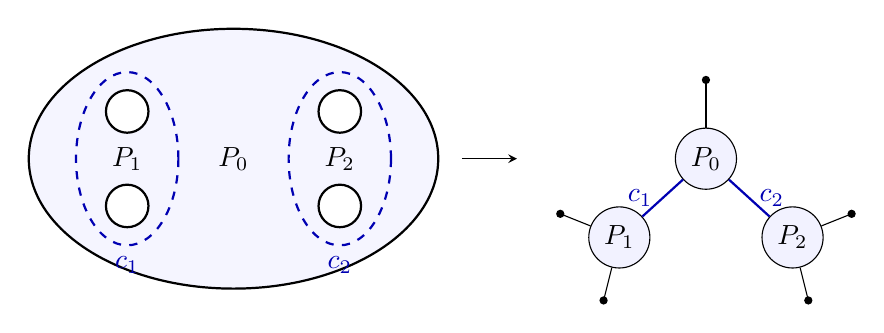
\begin{tikzpicture}[x=1cm,y=1cm,>=stealth]
	\draw[thick,fill=blue!4] (0,0) ellipse (2.6 and 1.65);
	\foreach \x in {-1.35,1.35}{
		\draw[thick,fill=white] (\x,0.6) circle (0.27);
		\draw[thick,fill=white] (\x,-0.6) circle (0.27);
		\draw[blue!70!black,thick,dashed] (\x,0) ellipse (0.65 and 1.1);
	}
	\node at (0,0) {\(P_0\)};
	\node at (-1.35,0) {\(P_1\)};
	\node at (1.35,0) {\(P_2\)};
	\node[blue!70!black] at (-1.35,-1.35) {\(c_1\)};
	\node[blue!70!black] at (1.35,-1.35) {\(c_2\)};
	\draw[->] (2.9,0)--(3.6,0);
	\begin{scope}[shift={(6,0)}]
		\node[circle,draw,fill=blue!5,inner sep=3pt] (p0) at (0,0) {\(P_0\)};
		\node[circle,draw,fill=blue!5,inner sep=3pt] (p1) at (-1.1,-1) {\(P_1\)};
		\node[circle,draw,fill=blue!5,inner sep=3pt] (p2) at (1.1,-1) {\(P_2\)};
		\draw[blue!70!black,thick] (p0)--node[left] {\(c_1\)}(p1);
		\draw[blue!70!black,thick] (p0)--node[right] {\(c_2\)}(p2);
		\draw (p0)--(0,1);
		\draw (p1)--(-1.85,-0.7);
		\draw (p1)--(-1.3,-1.8);
		\draw (p2)--(1.85,-0.7);
		\draw (p2)--(1.3,-1.8);
		\foreach \x/\y in {0/1,-1.85/-0.7,-1.3/-1.8,1.85/-0.7,1.3/-1.8}{
			\fill (\x,\y) circle (1.5pt);
		}
	\end{scope}
\end{tikzpicture}

	\caption[五边界球面的裤分解]{从五边界球面依次切下两条裤子，最后留下第三条。右图记录三个裤形分支的邻接关系：两个内部接缝各对应一条切割曲线，五个外端分别对应原来的五条边界。图记录拓扑粘合，不预设长度或角度。}
	\label{g1:fig:pants-tree}
\end{figure}

例如，闭的亏格 \(2\) 曲面需要 \(3\) 条切口，得到 \(2\) 条裤子；一次穿孔环面需要 \(1\) 条切口，得到 \(1\) 条裤子；五边界球面需要 \(2\) 条切口，得到 \(3\) 条裤子，如\cref{g1:fig:pants-tree}。恢复原曲面时，同一条裤子的两条边界可以彼此粘合，切口两侧因而可能属于同一块裤形曲面。

\ProseParagraphBreak

条件 \(\chi<0\) 来自每块裤形曲面的负 Euler 示性数。球面、圆盘、环带和闭环面分别有 Euler 示性数 \(2,1,0,0\)，沿闭曲线切开仍保持该数，因而不可能变成非空的裤形曲面之并。闭环面可以沿一条经线切成环带，但环带不是裤子。另一方面，裤形曲面本身满足 \(\chi=-1\)，其分解使用 \(0\) 条切口，符合公式，给出允许空曲线组的基本例子。

\ProseParagraphBreak

裤分解为后面的双曲几何提供了一个清楚的粘合问题：先给每条裤子配置适当的几何结构，再把对应边界按相容的数据接回去。拓扑分解记录块数与连接圆周；选定双曲几何结构后，边界长度与粘合扭转才成为新的数据。双曲裤子的存在与唯一性、边界长度的作用以及粘合中的扭转参数，都需要后卷的度量与测地线理论。这里已经确定的是分成多少块、沿哪些圆周连接，以及这些切口怎样反映曲面的亏格和边界。
% 纲要条目排为编号小节标题，并进入目录与 PDF 书签；说明段仍保留于纲要注释中。


\begin{chaptersummary}
	内点和边界点由局部拓扑区分；紧曲面只有有限个连通分支，边界是有限个圆周的不交并。平面同胚对小环路绕数的作用给出方向符号，符号在换图下相乘，由此定义局部定向、曲面定向与定向二叶覆盖。

	\ProseParagraphBreak

	Jordan 分离定理给出闭曲线的两侧，Schoenflies 延拓进一步把两侧的闭区域变成圆盘。简单弧直化和有限图邻域随后使圆盘边界能够逐个正则化，形成有限盘形分解并三角化。不同拓扑剖分的边可能无限相交，因此先通过环境同痕整理，再取公共细分；细分的局部计数证明 Euler 数与剖分无关。

	\ProseParagraphBreak

	对偶生成树把三角形粘成一个多边形；在闭曲面中再配合原骨架的生成树，可以得到一个顶点圆盘、有限条带和一个补圆盘。扭带抽出交叉帽，交错的无扭带抽出手柄；每次带数减少，约化因而终止。一个手柄与一个交叉帽可改写为三个交叉帽，这使不可定向情形归于统一模型。边界先封盘、最后恢复，圆盘搬移保证挖孔位置不会另添分类参数。

	\ProseParagraphBreak

	紧连通曲面恰为 \(\Sigma_{g,b}\) 或 \(N_{k,b}\)，其中前者可定向，后者不可定向。它们的 Euler 示性数分别为 \(2-2g-b\) 和 \(2-k-b\)；结合边界分支数与可定向性，即可唯一恢复参数。基本群展示检验这些模型中的环路和关系，但带边界曲面的自由基本群单独不足以完成分类。

	\ProseParagraphBreak

	简单闭曲线有环带或 Möbius 带邻域，沿曲线切开保持 Euler 示性数，改变边界数，并可能改变连通性与可定向性。负 Euler 示性数的可定向紧曲面可以分成裤子：\(\Sigma_{g,b}\) 的裤子数为 \(2g-2+b\)，切口数为 \(3g-3+b\)。这些是拓扑分解；在它们上面选择长度、扭转和双曲度量，还需要后续的几何论证。
\end{chaptersummary}

\BookExercises
以下各题均附完整解答。辨认曲面时先说明紧性、连通性、边界数与可定向性；使用 Euler 数前确认所用分解的面是圆盘；切割问题还需说明切口两侧怎样接回。


\begin{exercise}\label{g1:ex:surface-intrinsic-boundary}
	分别将闭圆盘 \(D^2\)、圆环 \(A=\{z\in\mathbb C:1\le |z|\le2\}\) 视为平面子集，将 \(S^2\) 视为三维空间子集。求各自的曲面边界及环境中的子集边界。说明开圆盘虽在平面中有圆周作为子集边界，却没有曲面边界；再说明本章为什么不把它称为闭曲面。
\end{exercise}
\begin{solution}
	闭圆盘的曲面边界与平面子集边界均为 \(S^1\)。圆环的两种边界均为 \(\{|z|=1\}\sqcup\{|z|=2\}\)。球面的每点都有平面圆盘图，所以曲面边界为空；它在 \(\mathbb R^3\) 中闭且内部为空，因此其环境边界是整个球面。

	开圆盘的每个点都有足够小的平面开圆盘邻域，所以没有曲面边界。它在 \(\mathbb R^2\) 中的闭包是闭圆盘，减去自身得到环境边界 \(S^1\)，但这些点不属于这个曲面。开圆盘不紧，例如递增开集 \(\{|z|<1-1/n\}\)、\(n\ge2\)，覆盖它却没有有限子覆盖。闭曲面要求紧且无曲面边界，因此开圆盘不满足前一条件。
\end{solution}

\begin{exercise}\label{g1:ex:wedge-disks-not-surface}
	把两张闭圆盘的中心识别为同一个点 \(p\)，其他点不识别，所得商空间为 \(X\)。证明 \(X\) 紧且 Hausdorff，但不是允许带边界的拓扑曲面。比较把两张圆盘沿整个边界逐点粘合的结果。
\end{exercise}
\begin{solution}
	有限个紧圆盘的不交并紧，故其商紧。不同于 \(p\) 的点可在原圆盘中取避开中心的相对开邻域；同一圆盘中的两点可按平面分开，不同圆盘中避开中心的邻域天然不交。把 \(p\) 与另一点分开时，在两张圆盘的中心各取小圆盘的并，另一个点取避开它们的邻域。这些集合均饱和，所以它们的像在商中开，证明 Hausdorff。

	\(X\setminus\{p\}\) 恰有来自两张圆盘的两个不交开闭部分。每个 \(p\) 的邻域都遇到两者，所以删去 \(p\) 后都不连通。但无论圆盘内点还是半圆盘直边中点，都有一个删去中心后仍道路连通的坐标邻域。这一必要局部性质失败，因此 \(X\) 不是曲面。

	沿整个边界粘合的情形不同。把两张圆盘分别映到上下闭半球，公共边界按同一赤道参数识别，便得到到 \(S^2\) 的连续双射；紧到 Hausdorff 的判据使它为同胚。赤道附近两个半圆盘共同组成圆盘邻域，并未产生前面的局部分叉。
\end{solution}

\begin{exercise}\label{g1:ex:orientation-pullback-cover}
	设 \(p:E\to M\) 是覆盖，\(M\) 是已定向的拓扑曲面，且 \(E\) 为 Hausdorff、第二可数。证明覆盖片使 \(E\) 成为拓扑曲面，并给出一个使 \(p\) 局部保持定向的唯一提升定向。证明任一甲板变换保持此定向。
\end{exercise}
\begin{solution}
	把 \(M\) 的坐标图缩到均匀覆盖邻域内；每张覆盖片经 \(p\) 同胚地映到该邻域，再接底空间坐标便得到 \(E\) 的圆盘或半圆盘图。题设已经给出两项整体拓扑条件，故 \(E\) 为曲面。

	在每张这样的提升图上采用底图的定向符号。两张提升图交叠时，坐标变换就是对应底图的坐标变换，所以相容关系成立。若要求 \(p\) 局部保持定向，任一点的符号就必须是这个符号，因此唯一。甲板变换 \(T\) 满足 \(pT=p\)，在上述坐标中，它只是从一张片移到另一张片而保持坐标值不变，局部方向符号为 \(1\)，故保持提升定向。
\end{solution}

\begin{exercise}\label{g1:ex:oscillating-edges}
	在平面中考虑两条简单弧
	\[
		A=\{(x,0):0\le x\le1\},\qquad B=\{(x,f(x)):0\le x\le1\},
	\]
	其中 \(f(0)=0\)，\(f(x)=x^2\sin(1/x)\) 对 \(x>0\)。证明它们有无限多个交点，却都是拓扑线段。说明为什么把这两条弧原样保留为边的两个有限剖分不可能有有限公共细分。最后给出一个局部环境同痕，把 \(B\) 的一个内点附近的短段直化。
\end{exercise}
\begin{solution}
	投影到第一坐标是每条弧到 \([0,1]\) 的连续双射，其逆分别是 \(x\mapsto(x,0)\)、\(x\mapsto(x,f(x))\)，因而两条弧都是拓扑线段。交点包含 \((1/(k\pi),0)\)，其中 \(k\ge1\)，这些点两两不同并趋近原点；它们没有构成公共线段，因为 \(f\) 不在任何正长度区间上恒为零。

	在一个有限单纯复形中，两条作为子复形的边链的交集仍为子复形。如果交集不含一条边，它就只能是有限个顶点。这里交集有无限多个孤立点且没有弧段，故不可能成为有限公共细分中的交集。这指出了“叠放两剖分即可细分”所缺少的有限性。

	取内点 \(x_0\in(0,1)\) 及一个小区间 \(J\) 包含 \(x_0\)。在竖直方向上用映射 \((x,y)\mapsto(x,y-tf(x))\) 即可把该段图像连续移到水平线；若要让修改有局部支撑，先在一条包含图像的窄矩形带中使用\cref{g1:lem:proper-arc-straightening}，得到固定矩形边界、把中线图像移到指定直径的同胚，再用\cref{g1:lem:graph-small-isotopy}证明中的圆盘公式把它连到恒等映射。这样修改只发生在指定带内，且每一时刻都是整个邻域的同胚。
\end{solution}

\begin{exercise}\label{g1:ex:double-euler}
	设 \(M\) 是紧曲面，边界非空，\(\widehat M\) 是沿边界粘合两个副本得到的双倍。直接用与边界相容的三角剖分证明 \(\chi(\widehat M)=2\chi(M)\)。分别对闭圆盘和圆环核对所得结果。
\end{exercise}
\begin{solution}
	记 \(M\) 的顶点、边、三角形数为 \(V,E,F\)，边界中的顶点数和边数为 \(V_\partial,E_\partial\)。两份副本粘合后，边界顶点和边界边各成对识别，三角形不识别，因此
	\[
		\chi(\widehat M)=(2V-V_\partial)-(2E-E_\partial)+2F
		=2\chi(M)-(V_\partial-E_\partial).
	\]
	每个边界分支是有限圈，顶点数等于边数，所以括号为零。双倍粘合得到的有限三角形分解若暂有重边，重心细分不改变交替和，故上述计数仍给出 \(\chi(\widehat M)\)。

	闭盘可取一个三角形，故 \(\chi(D^2)=3-3+1=1\)，双倍是两个盘沿圆周相接的球面，其 Euler 数为 \(2\)。圆环取内、外两圈各 \(m\ge3\) 个顶点，连接对应顶点，并把每个四边形沿一条对角线分开，得到 \(2m\) 个顶点、\(4m\) 条边和 \(2m\) 个三角形，交替和为 \(0\)。圆环双倍是环面，Euler 数仍为 \(0\)。
\end{solution}

\begin{exercise}\label{g1:ex:disk-two-marked-points}
	设 \(B,B'\) 是闭 Jordan 盘，\(f:\partial B\to\partial B'\) 是同胚，\(p\in B^\circ\)、\(p'\in B'^\circ\)。证明 \(f\) 有一个把 \(p\) 送到 \(p'\) 的闭盘同胚延拓。再证明，固定闭盘边界的任意同胚都与恒等映射经固定边界的环境同痕相连。
\end{exercise}
\begin{solution}
	先由\cref{g1:thm:jordan-schoenflies}延拓为 \(F:B\to B'\)，记 \(q=F(p)\)。把 \(B'\) 同胚到一个正方形，把 \(q,p'\) 的像分别向四个角连线，得到两个具有相同组合关系的扇形三角剖分。在对应三角形上取仿射同胚，它们在公共半径上相合且在正方形边界上恒等，因而粘成一个固定边界、把 \(q\) 的像送到 \(p'\) 的像的同胚。共轭回 \(B'\)，再与 \(F\) 复合即得所求。

	第二问把盘识别为单位圆盘，使用正文的缩放公式 \(U_t(x)=tu(x/t)\)（\(\|x\|\le t\)）以及 \(U_t(x)=x\)（\(\|x\|\ge t\)）。每个 \(U_t\) 固定边界，逆由 \(u^{-1}\) 的同一公式给出；\(\|U_t(x)-x\|\le2t\) 保证 \(t\to0\) 的连续性。于是得到固定边界的同痕。注意这个结论要求原同胚在边界上逐点恒等；反射圆盘的同胚不满足这一条件。
\end{solution}

\begin{exercise}\label{g1:ex:relative-triangulation-euler}
	设紧曲面 \(M\) 上嵌入了一个有限图 \(G\)，图与边界相容，且所有补区域都是开圆盘，每条边的两侧允许属于同一补区域。说明为什么能够选一个以 \(G\) 为子复形的有限三角剖分。若某补区域的边界行走重复经过顶点或边，为什么不能直接给这条边界行走加一个中心点并声称得到单纯复形？用环面的标准一顶点、两条环边、一张方形面的分解计算 Euler 数，并说明与真正三角剖分的联系。
\end{exercise}
\begin{solution}
	由\cref{g1:thm:surface-triangulation}的相对形式，先把 \(G\) 加入有限曲线网，再作顶点盘、边矩形和补区域的圆盘化，即可保留 \(G\) 并得到有限三角剖分。添加的顶点只把原边分成有限段，所以 \(G\) 成为一个子复形。

	如果边界行走把同一顶点访问两次，则从中心连出的两条半径可能有相同端点而是不同的边；如果同一边出现两次，同一个三角形的不同边也可能在商空间中识别。单纯复形由顶点集合唯一确定单形，因而这种未经处理的扇形画法只给出三角形粘合描述。先取顶点盘与边矩形，再细分这些盘形块，才能得到符合定义的三角剖分。

	环面的方形分解有 \(V=1,E=2,F=1\)，所以交替和为 \(0\)。为把这个计数与正式定义联系起来，可在方形上取 \(m\times m\) 方格并沿同向对角线分割，其中 \(m\ge3\)，然后识别相对边。商中有 \(m^2\) 个顶点、\(3m^2\) 条边和 \(2m^2\) 个三角形，确为单纯复形，交替和仍为 \(m^2-3m^2+2m^2=0\)。粗分解虽然便于计算，细分则说明这个数确实是环面的 \(\chi\)。
\end{solution}

\begin{exercise}\label{g1:ex:tetrahedron-two-trees}
	用四面体边界作为球面剖分，顶点为 \(0,1,2,3\)。选原骨架的生成树 \(T=\{01,02,03\}\)。写出不穿 \(T\) 的对偶生成树，并指出顶点圆盘加带条模型中剩多少条带条。
\end{exercise}
\begin{solution}
	四个面分别为 \(012,013,023,123\)。未在 \(T\) 中的边是 \(12,13,23\)；它们的对偶边分别连接 \(123\) 与 \(012,013,023\)。因此这三条对偶边是一棵以面 \(123\) 为中心的星形生成树。六条原边已经分别被 \(T\) 或对偶树使用，没有剩余带条。于是两个树的盘状邻域分别形成顶点盘与面盘，沿唯一圆周粘合，得到球面。整个构造直接给出了球面模型，而没有先用 Euler 数判别。
\end{solution}

\begin{exercise}\label{g1:ex:two-letter-polygons}
	对边字 \(aabb\) 和 \(abab^{-1}\)，分别追踪四个角的等价类，计算相应胞腔分解的 \(v-e+f\)。再与 \(aa^{-1}bb^{-1}\) 比较。这里尚不要求只凭这些整数判断前两张曲面的同胚类型。
\end{exercise}
\begin{solution}
	依边界顺序写角为 \(v_0,v_1,v_2,v_3\)。对 \(aabb\)，两条 \(a\) 同向配对给出 \(v_0=v_1=v_2\)，两条 \(b\) 的配对再令 \(v_2=v_3=v_0\)，所以只有一个顶点。对 \(abab^{-1}\)，\(a\) 的同向配对给出 \(v_0=v_2,v_1=v_3\)，而 \(b\) 的反向配对给出 \(v_1=v_0,v_2=v_3\)，同样只有一个顶点。两者均有两条商边、一张面，所以 \(v-e+f=1-2+1=0\)。

	对于 \(aa^{-1}bb^{-1}\)，正文已追踪出三个顶点，仍有两条边和一张面，故为 \(3-2+1=2\)。这说明“一个四边形、两对边”不足以确定 Euler 数，顶点等价关系不可省略。前两张曲面最终都属于不可定向的两交叉帽模型，但这一同胚还须靠后面的合法切粘或分类证明，而不是由相同整数单独断言。
\end{solution}

\begin{exercise}\label{g1:ex:capping-parameter}
	设 \(M\) 为紧曲面，\(C\) 为其一个边界圆周，\(h_0,h_1:S^1\to C\) 为两个同胚。显式构造两个封口空间 \(M\cup_{h_0}D^2\) 与 \(M\cup_{h_1}D^2\) 之间在 \(M\) 上恒等的同胚，并说明为何即使 \(h_0,h_1\) 在圆周上的方向相反也成立。
\end{exercise}
\begin{solution}
	在圆盘边界上取 \(k=h_1^{-1}h_0\)，径向延拓为 \(K(ru)=r k(u)\)、\(K(0)=0\)。在不交并 \(M\sqcup D^2\) 上，令映射在 \(M\) 上恒等、在圆盘上为 \(K\)。源空间中 \(u\sim h_0(u)\)，而目标空间中 \(K(u)=h_1^{-1}h_0(u)\sim h_0(u)\)，故它尊重识别，下降为连续映射。用 \(K^{-1}\) 得到逆映射，所以是同胚。

	径向延拓只要求 \(k\) 是圆周同胚，不要求保向。如果两个封口参数方向相反，\(K\) 就反转所添圆盘的方向，但并不改变未预先定向的封口曲面。若另要求封口后延续一个给定的曲面定向，则应在新圆盘上选择相应方向；这是附加的定向资料问题。
\end{solution}

\begin{exercise}
	用合法切粘识别边字 \(abab\) 与 \(aba b^{-1}\) 给出的闭曲面；说明为何不能只数它们都有两种字母，就认定是同一个模型。
\end{exercise}
\begin{solution}
	对 \(abab\)，在\cref{g1:eq:crosscap-word-move}取 \(U=b\)、\(V=b\)，得到 \(xxb^{-1}b\)。相邻反向边 \(b^{-1}b\) 可按\cref{g1:prop:polygon-moves}消去，余字 \(xx\) 给出 \(\mathbb RP^2=N_{1,0}\)。这里消去后仍有 \(xx\)，不涉及把球面的退化双边形误看成空空间的问题。

	对 \(abab^{-1}\)，同样取 \(U=b\)、\(V=b^{-1}\)，得到 \(xxb^{-1}b^{-1}\)。将 \(b^{-1}\) 重标为 \(y\)，便是 \(xxyy\)，故为 \(N_{2,0}\)，也就是 Klein 瓶。两份 \(b\) 的方向不同，改变了端点识别与可抽出的带条数据。边字中的字母数还可能因原来有多个顶点或相邻可消边而冗余，必须连同全部配对规则一起使用。
\end{solution}

\begin{exercise}
	对有边界曲面也可在内部各取一个盘作连通和。证明
	\[
		\Sigma_{g,b}\#\Sigma_{h,c}\cong\Sigma_{g+h,b+c},\qquad
		\Sigma_{g,b}\#N_{k,c}\cong N_{2g+k,b+c},\qquad
		N_{k,b}\#N_{\ell,c}\cong N_{k+\ell,b+c}.
	\]
	其中 \(g,h,b,c\ge0\)，\(k,\ell\ge1\)。说明这些构造不需要先使用下一节的 Euler 数公式。
\end{exercise}
\begin{solution}
	先将原有的 \(b+c\) 条边界全部封盘，再在避开这些盘的位置作连通和。由于取盘及粘合都可与所封的盘保持不交，最后去掉原补盘就恢复带边界的连通和；\cref{g1:lem:disk-configuration}保证这些余孔的位置不影响模型。因此只需计算闭模型，最后保留 \(b+c\) 个孔。

	两种可定向模型的边字都是交换子串，将字串接就有 \(g+h\) 个交换子，给出 \(\Sigma_{g+h,0}\)。两种不可定向模型的平方字串接，得到 \(k+\ell\) 个平方，给出 \(N_{k+\ell,0}\)。混合情形先得到 \(g\) 个手柄与 \(k\) 个交叉帽；因为 \(k\ge1\)，可连续 \(g\) 次使用\cref{g1:lem:handle-crosscap-trade}，每次把一个手柄及一个已有交叉帽换成三个交叉帽，最终有 \(2g+k\) 个交叉帽。整个论证逐步构造同胚，没有借助同胚不变量倒推模型。
\end{solution}

\begin{exercise}
	在圆盘上粘四条无扭带，八个粘合区间沿边界依次为 \(a,b,c,d,d,c,b,a\)。证明带面有五条边界；沿全部五条边界分别补盘后得到球面。由此说明“四条无扭带应当是两个手柄”的推断漏掉了什么条件。
\end{exercise}
\begin{solution}
	先只粘最内侧的 \(d\) 带。它的两个端区间之间没有其他端点，因此它的一条长边与这段盘边界形成一个新圆周，另一侧仍承载 \(a,b,c\) 的全部端点。再粘 \(c\) 带时，其两个端点在承载剩余端点的同一条边界上相邻，又分出一个没有其他端点的新圆周。\(b\)、\(a\) 两带同理。每加一条带，边界数增加一；从圆盘的一条边界出发，最终有五条。

	把每次分出的那条新圆周立即封盘。该带、所封圆盘和盘边界之间的小区域合在一起，只是把原盘沿一个边界弧向外扩大：沿横穿带的一条弧切开，可看成两盘沿整条边粘合，因而仍是盘。四次如此消去四条带，最后余下一个盘；再封住它唯一的边界，得到两盘沿圆周粘合的球面。

	抽取手柄的命题要求余带面只有一条边界，并且两条无扭带的端点交错。本题没有交错边对，也没有单边界条件，不能把带数直接除以二当作手柄数。
\end{solution}

\begin{exercise}
	设 \(M\) 是闭连通曲面，\(p_1,\ldots,p_b\) 是互异点，\(b\ge1\)。证明 \(M\setminus\{p_1,\ldots,p_b\}\) 形变收缩到一个从 \(M\) 去掉 \(b\) 个内开盘所得的紧曲面，但二者并不同胚。
\end{exercise}
\begin{solution}
	取互不相交的闭坐标盘 \(D_i\)，在每个盘的单位圆盘坐标中令 \(p_i\) 对应原点。对 \(0<r\le1\)，定义
	\[
		H_s(ru)=((1-s)r+s)u,\qquad u\in S^1,\quad 0\le s\le1.
	\]
	在各 \(D_i\setminus\{p_i\}\) 上使用此公式，在全部盘外保持不动。公式在 \(r=1\) 上固定，所以与盘外恒等映射相容，给出连续形变收缩，其终像为 \(M\setminus\bigcup_i\operatorname{int}D_i\)。

	这个终像是闭曲面 \(M\) 的闭子集，因而紧。去点空间不紧：若它紧，由 \(M\) 为 Hausdorff，它应为 \(M\) 的闭子集；但在任一被去点的坐标盘中，非中心点趋近中心，说明该去点空间不闭。因此两者不能同胚。这里的形变收缩只保证同伦类型相同，不保留紧性或流形的边界。
\end{solution}

\begin{exercise}\label{g1:ex:surface-cover-genus}
	\begin{enumerate}
		\item 设 \(p:T\rightarrow\Sigma_{g,0}\) 是连通 \(d\) 叶覆盖。证明 \(T\) 可定向，并计算其亏格。当 \(g=0\) 时，说明这限制了哪些 \(d\)。
		\item 一个连通三叶覆盖以一次穿孔环面为底空间，若边界环路在三点纤维上的单值是一个三循环，确定总空间的同胚类型。
	\end{enumerate}
\end{exercise}
\begin{solution}
	(1) 将底空间的定向通过覆盖片提起，坐标变换仍保持定向，故 \(T\) 可定向。有限覆盖的总空间紧，且底空间无边界，覆盖的局部模型也没有边界。若 \(T=\Sigma_{h,0}\)，则 \(2-2h=d(2-2g)\)，所以 \(h=1+d(g-1)\)。当 \(g=0\) 时，\(h=1-d\ge0\) 迫使 \(d=1\)，这与球面单连通、没有非平凡连通覆盖相符。

	(2) 底空间可定向，故总空间可定向；由 \(\chi(\Sigma_{1,1})=-1\)，得到 \(\chi(T)=-3\)。边界上方的连通分支对应边界环路在纤维上的轨道，一个三循环只有一个轨道，所以 \(T\) 只有一条边界。于是 \(2-2h-1=-3\)，得 \(h=2\)，即 \(T\cong\Sigma_{2,1}\)。这个单值条件可以实现：在 \(F_2=\langle a,b\rangle\) 上令 \(a,b\) 分别作换位 \((12),(23)\)，它们生成传递作用，而交换子作三循环；根据正文的展示，边界环路是交换子的逆，也仍作三循环。覆盖重建定理因而确实给出一个这样的连通覆盖。
\end{solution}

\begin{exercise}\label{g1:ex:surface-invariant-recovery}
	对下列数据，确定所有符合条件的紧连通曲面，或证明不存在：
	\begin{enumerate}
		\item 有两条边界，Euler 示性数为 \(-4\)，未说明可定向性。
		\item 无边界且可定向，Euler 示性数为 \(-3\)。
		\item 有一条边界，定向覆盖连通且同胚于 \(\Sigma_{3,2}\)。
	\end{enumerate}
\end{exercise}
\begin{solution}
	(1) 可定向时，\(2-2g-2=-4\)，故 \(g=2\)，得到 \(\Sigma_{2,2}\)。不可定向时，\(2-k-2=-4\)，故 \(k=4\)，得到 \(N_{4,2}\)。二者都存在，并因可定向性不同而不同胚。

	(2) 闭可定向曲面的示性数 \(2-2g\) 为偶数，不能为 \(-3\)，故不存在。

	(3) 定向覆盖连通说明底曲面不可定向。覆盖总空间的示性数为 \(2-6-2=-6\)，二叶性给出底空间示性数为 \(-3\)。代入 \(2-k-1=-3\)，得 \(k=4\)，所以底曲面为 \(N_{4,1}\)；其定向覆盖公式也恰给出 \(\Sigma_{3,2}\)。
\end{solution}

\begin{exercise}\label{g1:ex:surface-abelianization-test}
	设 \(G=\langle a,b,c\mid a^2b^2c^2=1\rangle\)。
	\begin{enumerate}
		\item 计算 \(G_{\mathrm{ab}}\) 及从 \(G\) 到 \(\mathbb Z/2\mathbb Z\) 的同态数。
		\item 找出一个与 \(G\) 的交换化有相同自由秩、但交换化不同构的闭可定向曲面群。
		\item 在 \(G\) 的七个非平凡同态 \(G\rightarrow\mathbb Z/2\mathbb Z\) 中，哪个核给出定向覆盖？该覆盖是什么曲面？
	\end{enumerate}
\end{exercise}
\begin{solution}
	(1) 交换化中只有关系 \(2a+2b+2c=0\)。以 \(u=a+b+c,b,c\) 为整数基，关系变成 \(2u=0\)，故 \(G_{\mathrm{ab}}\cong\mathbb Z^2\oplus\mathbb Z/2\mathbb Z\)。到 \(\mathbb Z/2\mathbb Z\) 时，原关系对三个生成元的任意像都成立，所以有 \(2^3=8\) 个同态。

	(2) 环面群的交换化是 \(\mathbb Z^2\)，自由秩同为 \(2\)，但没有非零二阶元素，故与上式不同构。

	(3) \(G\) 是 \(N_{3,0}\) 的群，三个标准交叉帽环路都反转定向。因此定向特征在加法记法下把 \(a,b,c\) 都送到 \(1\in\mathbb Z/2\mathbb Z\)。它非平凡，核的指数为 \(2\)，对应连通定向二叶覆盖。由定向覆盖公式，总空间为 \(\Sigma_{2,0}\)。其他六个非平凡同态也给出二叶覆盖，但不对应这个核；不能仅凭覆盖的叶数把它们认作定向覆盖。
\end{solution}

\begin{exercise}\label{g1:ex:capping-surface-group}
	设 \(S=\Sigma_{g,b}\) 或 \(N_{k,b}\)，且 \(b\ge1\)。沿其中一条边界封上圆盘。说明包含同态在基本群上的核，并以一次穿孔环面与 Möbius 带为例，分别写出封盘前后的群。
\end{exercise}
\begin{solution}
	将被封边界的环路用连接道路带到基点，记其类为 \(d\)。封盘正是沿该边界附着一个圆盘，故由\cref{g1:prop:attach-disk}，包含同态满射，核为 \(\langle\!\langle d\rangle\!\rangle\)。改变连接道路只把 \(d\) 共轭，改变方向只把它取逆，都不改变这个正规闭包。

	一次穿孔环面的群为 \(F_2=\langle a,b\rangle\)，边界类可取 \([a,b]^{-1}\)；封盘后加入 \([a,b]=1\)，得到 \(\mathbb Z^2\)，即闭环面群。Möbius 带的群为 \(\langle c\rangle\cong\mathbb Z\)，其边界类为 \(c^{-2}\)；封盘后加入 \(c^2=1\)，得到 \(\mathbb Z/2\mathbb Z\)，即实射影平面群。第二个例子还表明，边界圆周的一个生成元不必映成曲面群的原始生成元。
\end{solution}

\begin{exercise}\label{g1:ex:genus-two-cuts}
	在闭可定向亏格 \(2\) 曲面上，分别构造一条非分离简单闭曲线和一条分离的本质简单闭曲线，确定两种切开曲面的类型，并说明两条曲线不可能被曲面的某个自同胚互相送到对方。
\end{exercise}
\begin{solution}
	把曲面看成两个环面的连通和。在其中一个手柄上取经线，同一手柄的纬线只横穿它一次，所以经线非分离；切开后为 \(\Sigma_{1,2}\)。再取连通和接缝附近的中心圆周，它把两个手柄分开，切开后为两个 \(\Sigma_{1,1}\)。这两个分支都不是圆盘或环带，故接缝是本质曲线。自同胚给出相应补集之间的同胚，必须保持补集连通分支数；前者补集连通，后者有两个分支，所以不可能互相送到对方。
\end{solution}

\begin{exercise}\label{g1:ex:klein-curve-types}
	把 Klein 瓶写成两个 Möbius 带沿边界的并，选其中一条中心曲线 \(a\)，再选两带的公共边界 \(c\)。
	\begin{enumerate}
		\item 判断 \(a,c\) 的一侧或两侧、分离或非分离，并确定切开后的曲面。
		\item 用展示 \(\langle u,v\mid u^2v^2=1\rangle\) 证明 \(c\) 在基本群中非平凡，却不是本节约定的本质曲线。
	\end{enumerate}
\end{exercise}
\begin{solution}
	(1) \(a\) 是一侧曲线，所以非分离；切开第一条 Möbius 带的中心后，余下部分为一条边界领圈，接到另一条 Möbius 带上不改变后者的类型，因此总的切开曲面仍为 Möbius 带。也可由 \(\chi=0\)、一条新边界及仍含另一条一侧曲线，恢复 \(N_{1,1}\)。公共边界 \(c\) 有来自两条带各一半的环形邻域，故为两侧曲线，切开后是两条 Möbius 带，所以分离。

	(2) 取 \(u,v\) 为两条带的中心生成元，\(c\) 的类是 \(u^2\) 或其逆、共轭。定义到加法群 \(\mathbb Z\) 的同态 \(u\mapsto1,v\mapsto-1\)，则关系 \(u^2v^2\) 映为 \(2-2=0\)，同态良定义，而 \(u^2\) 映为 \(2\ne0\)。所以 \(c\) 非平凡。它却围出嵌入 Möbius 带，按本节约定被排除在本质曲线之外。这说明不可定向情形必须读清“本质”的具体定义。
\end{solution}

\begin{exercise}\label{g1:ex:pants-dual-graph}
	设 \(\Sigma_{g,b}\) 满足 \(\chi<0\)，给定一个裤分解。作一个有限图：每条裤子给一个顶点，每条切口给一条连接其两侧裤子的边，允许环边；原边界只作标记，不计作边。证明这个图连通，其基本群为 \(F_g\)。分别描述一次穿孔环面和闭亏格 \(2\) 曲面可能出现的图。
\end{exercise}
\begin{solution}
	原曲面连通，若裤子的邻接图分成两部分且没有连边，则把每部分的裤子按其内部接缝粘合后，得到原曲面的两个不交非空开闭部分，矛盾。因此图连通。顶点数 \(P=2g-2+b\)，边数 \(C=3g-3+b\)，由有限图的基本群公式，
	\[
		\pi_1(\text{邻接图})\cong F_{C-P+1}=F_g.
	\]
	一次穿孔环面只有一条裤子和一条切口，所以图是一个顶点加一条环边，剩下一条裤子边界作原边界标记。闭亏格 \(2\) 曲面有两个顶点、三条边，可以取三条边都连接这两个顶点的图：把两条裤子的三对边界分别粘合即可。也可以各在一个顶点添一条环边，再用第三条边连接两个顶点，这对应先把每条裤子的一对边界自粘成一次穿孔环面，再沿剩余边界粘合。两图都连通且边数减顶点数加一为 \(2\)，但它们的边与曲面内分离曲线的对应有所不同。
\end{solution}

\begin{exercise}\label{g1:ex:one-sided-cut-orientation}
	设 \(c\) 是 \(N_{k,b}\) 内的一侧简单闭曲线。证明：
	\begin{enumerate}
		\item 若切开后不可定向，则切开曲面为 \(N_{k-1,b+1}\)，并且 \(k\ge2\)。
		\item 若切开后可定向，则 \(k\) 为奇数，切开曲面为 \(\Sigma_{(k-1)/2,b+1}\)。
		\item 分别给出切开后不可定向、可定向的具体例子，说明一侧曲线不能只凭“删去一个交叉帽”这句话判断余下曲面的定向性。
	\end{enumerate}
\end{exercise}
\begin{solution}
	一侧切开后连通，边界数为 \(b+1\)，Euler 示性数仍为 \(2-k-b\)。若所得曲面为 \(N_{r,b+1}\)，则 \(2-r-(b+1)=2-k-b\)，所以 \(r=k-1\)，不可定向要求 \(r\ge1\)，即 \(k\ge2\)。若所得曲面为 \(\Sigma_{h,b+1}\)，则 \(2-2h-(b+1)=2-k-b\)，故 \(2h=k-1\)，得到第二项。

	第三项的不可定向例子是 Klein 瓶中一个交叉帽的中心曲线：切开后为 Möbius 带。可定向例子可取实射影平面中的射影直线，它是 Möbius 带的中心，切开后为圆盘。还有亏格较高的例子：把一次穿孔环面与 Möbius 带沿边界粘合，由\cref{g1:lem:handle-crosscap-trade}得到 \(T^2\#\mathbb RP^2\cong N_{3,0}\)；沿这条 Möbius 带的中心切开，余下的薄领圈只把一次穿孔环面的边界向外移，所得仍为 \(\Sigma_{1,1}\)。同样在 \(N_{3,0}\) 的三个交叉帽标准模型中，沿一个标准交叉帽中心切开却得到 \(N_{2,1}\)。可见余下曲面是否可定向取决于这条曲线的具体位置。
\end{solution}
